%\do\gammaumentclass[reqno]{amsart}
\documentclass[11pt]{article}

\usepackage{a4wide}
\usepackage{amsmath,amssymb,amsthm,amscd}
\usepackage[pdftex]{graphicx}

%\usepackage{showkeys}

\usepackage[all]{xy}

\newcommand{\bb}[1]{\begin{equation}\label{#1}}
\newcommand{\ee}{\end{equation}}
\newcommand{\vc}[1]{{\bf #1 }}
\renewcommand{\vec}[1]{{\bf #1}}
\newcommand{\Sum}[1]{\sum\limits_{#1}}
\newcommand{\Int}[1]{\int\limits_{#1}}
\newcommand{\Prod}[1]{\prod\limits_{#1}}
\newcommand{\const}{\operatorname{const}}
\newcommand{\ul}{\underline}
\newcommand{\ol}{\overline}
\newcommand{\tr}{\operatorname{tr}}
\newcommand{\bbA}{\mathbb A}
\newcommand{\bbR}{\mathbb R}
\newcommand{\bbN}{\mathbb N}
\newcommand{\bbZ}{\mathbb Z}
\newcommand{\bbC}{\mathbb C}
\newcommand{\bbT}{\mathbb T}
\newcommand{\QB}{\mathcal H}
\newcommand{\PQB}{\tilde{\mathcal H}}
\newcommand{\CQB}{\mathcal H'}
\newcommand{\Ad}{\operatorname{Ad}}
\newcommand{\ad}{\operatorname{ad}}
\newcommand{\gh}{\operatorname{gh}}
\newcommand{\Der}{\operatorname{Der}}
\newcommand{\Aut}{\operatorname{Aut}}
\newcommand{\aut}{\operatorname{aut}}
\newcommand{\Diff}{\operatorname{Diff}}
\renewcommand{\dim}{\operatorname{dim}}
\newcommand{\Vol}{\operatorname{Vol}}
\newcommand{\Pf}{\operatorname{Pf}}
\newcommand{\Cov}{\operatorname{Cov}}

\newcommand{\g}{{\bf g}}
\newcommand{\h}{{\bf h}}
\renewcommand{\d}{{\bf d}}
\newcommand{\e}{{\bf e}}
\renewcommand{\t}{{\bf t}}
\newcommand{\lpartial}{\overset{\rightarrow}{\partial}}
\newcommand{\rpartial}{\overset{\leftarrow}{\partial}}
\newcommand{\lder}[1]{\overset{\rightarrow}{\vc #1}}
\newcommand{\rder}[1]{\overset{\leftarrow}{\vc #1}}
\newcommand{\supp}{\operatorname{supp}}
\newcommand{\im}{\operatorname{Im}}
\renewcommand{\ker}{\operatorname{Ker}}
\newcommand{\Var}{\operatorname{Var}}




%define the \identy operator
\def\litID{{\sf id}}
\def\identy{{\mathsurround0pt\mathchoice{\textidenty}{\textidenty}{\scptidenty}{\scptidenty}}}
\def\scptidenty{\setbox0\hbox{$\scriptstyle1$}\bothidenty}
\def\textidenty{\setbox0\hbox{$1$}\bothidenty}
\def\bothidenty{\rlap{\hbox to.97\wd0{\hss\vrule height.06\ht0 width.82\wd0}}
 \copy0\rlap{\kern-.36\wd0\vrule height1.05\ht0 width.05\ht0}\kern.14\wd0}
%end of definition \identy
\newtheorem{theorem}{Theorem}[section]

\newtheorem{corollary}[theorem]{Corollary}

\newtheorem{definition}[theorem]{Definition}

\newtheorem{lemma}[theorem]{Lemma}

\newtheorem{lemmadefinition}[theorem]{Lemma and Definition}

\newtheorem{proposition}[theorem]{Proposition}

\theoremstyle{definition}

\newtheorem{example}[theorem]{Example}

\newtheorem{remark}[theorem]{Remark}



\newcommand{\bbM}{\mathbb M}
\newcommand{\bt}{\pmb\theta}
\newcommand{\Bt}{\pmb\Theta}

\begin{document}

\title{Boosting Bayesian Parameter Inference for Nonlinear Stochastic Differential Equation Models by Hamiltonian Scale Separation}

\author{Carlo Albert\footnote{Eawag, Swiss Federal Institute of Aquatic Science and Technology, 8600 D\"ubendorf, Switzerland}, Simone Ulzega\footnotemark[1], Ruedi Stoop\footnote{Institute of Neuroinformatics and Institute of Computational Science UZH/ETHZ, Irchel Campus 8057 Zurich, Switzerland}}

\maketitle

\begin{abstract}
We propose a novel very efficient approach for generating posterior parameter distributions, for the modeling of dynamical systems characterized by time-series. The algorithm is inspired by re-interpreting the posterior distribution as a partition function of a
%1D
statistical mechanics system. To arrive at distribution samples, we employ a Hamiltonian Monte Carlo approach combined with multiple time-scale integration.
At least for 1D problems, generic re-parametrization allows us to decouple the harmonic modes between measurement points and solve their dynamics analytically.
%Generic re-parametrization helps us to decouple the harmonic modes between measurement points, which leads to an analytical solution of the node dynamics.
Our approach is applicable to a wide range of inference problems and is highly parallelizable.


\end{abstract}


\section{Introduction}

Modeling a dynamical process starts with a basic model that is usually obtained from more or less deep insight into the nature of the process. The next step then is the determination of the parameters of the model, based on observed data, which is generally a highly nontrivial task, in particular when complex behavior of such systems needs to be predicted, or when the measurements are noisy.
A minimal example is a perceptron [XXX], the basic element of a neuronal network, that predicts the double cosine value associated with the input of the corresponding sine function plus the sine's value at a fixed earlier time. While this task can easily be achieved for clean data using gradient descent learning, for noisy input data this is largely impossible, as noise cannot be learned. The result is a distribution of potential parameter values (Fig.~(\ref{neural})).
\begin{figure}[h]
    \centering
    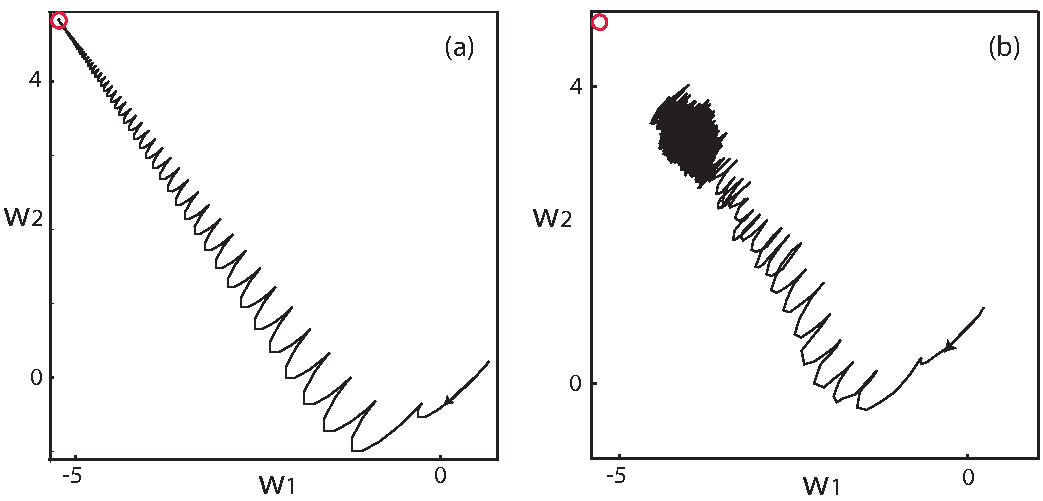
\includegraphics[width=1.0\textwidth]{neuron.pdf}
    \caption{General problem setting: Parameter estimation (synaptic weights $w_1$,$w_2$) of a perceptron, from a) noiseless, b) noisy data (noise sampled from a flat distribution over the  interval $[-0.2,0.2]$). Whereas for noiseless data the estimates perfectly converge, for noisy data the estimates  the system attempts to also include the noise, leading to a nontrivial distribution of the parameter estimates, and rendering the extraction of the optimal parameters a nontrivial task. Open circles: location of the optimal parameters in the noiseless case.}
    \label{neural}
\end{figure}

In Bayesian statistics, knowledge about parameters is expressed by probability distributions and learning is implemented as an update rule on these distributions [REF].
If a constant noise term is added to the output of a deterministic model, such as in the perceptron example above, Bayesian inference is straightforward.
If noise enters the formulation of the model equations, however, Bayesian inference all of a sudden becomes computationally very expensive.

In our paper, we demonstrate the calibration of ordinary 1D stochastic differential equation (SDE) models based on noisy time series, and the quantification of the resulting parametric uncertainty. The generic approach that we use is exemplified by a simple SDE model from hydrology.

%Bayesian parameter inference for SDE models is computationally very expensive, as the posterior parameter probability density is a path-integral.
Problems of this kind are commonly solved by Monte Carlo (MC) methods that are based on simulating model realizations and comparing them to the data. Popular methods are particle filters \cite{chopin_2013_SMC2}, Metropolis-within-Gibbs algorithms \cite{tomassini_2009_smoothing, reichert_2009_timedepParameters} or Approximate Bayes Computations (ABC) \cite{marin_2012_ABC, Albert_2014_ABC}.
A major problem with these simulation-based methods is, however, their inefficiency in the presence of many data points or high dimensions. One solution is to map the output space to a smaller dimensional space of summary statistics, and accept/reject proposed model parameters depending on how well associated model runs conform with the data in terms of these summary statistics [Ref.]. However, how to choose the summary statistics to achieve a significant representation of the posterior parameter distribution is a largely unsolved problem.

%In our approach we remedy these difficulties.
%We start by re-interpreting the posterior distribution as the partition function of a statistical mechanical system, of which we simulate the time evolution.
These difficulties can be remedied with a reinterpretation of the Bayesian posterior distribution as the partition function of a statistical mechanics system and by simulating the dynamics of the latter.
After discretizing the time of the original problem, we are led to the statistical mechanics of a polymer %-like problem
with harmonic bonds in an exterior potential. In this framework, the measurements are interpreted as an additional exterior potential that acts only on the polymer's `measurement beads', and model parameters are interpreted as additional degrees of freedom coupling to all the beads of the polymer.
To simulate the dynamics of this system, we apply the Hamiltonian Monte Carlo (HMC) algorithm \cite{duane_1987}, which combines Molecular Dynamics (MD) \cite{alder_1959_MD, rahman_1964_MD} with the Metropolis algorithm  \cite{metropolis_1953}.
Compared to traditional methods, the use of the Hamiltonian approach achieves much higher acceptance rates since data points are already used for the suggestion of new parameters, and thus model realizations incompatible with the data are never considered. The drawback is that the model equations need to be known and derivatives have to be calculated.

HMC requires two sets of parameters to be tuned: (i) the parameters that define the kinetic energy of the statistical mechanics system and (ii) the parameters that define the numerical integration scheme of Hamilton's equation in the molecular dynamics part of the HMC algorithm. Efficiency of HMC algorithms can be gained if the kinetic term is made dependent on the configuration geometry of the statistical mechanics system. If the Riemann geometry of the parameter space of statistical models is taken into account, then the simulated search of paths across this manifold samples the target density in an utmost efficient way
    \cite{girolami_2011_HMC}. Unfortunately, this procedure is both demanding and computationally costly,  depending strongly on the quality of the space's extracted geometry.


%Riemann geometry of the parameter space of statistical models and thus automatically adapts to the local structure when simulating paths across this manifold, providing highly efficient convergence and exploration of the target density

Here we
%therefore
explore a computationally simpler approach, which, to our knowledge, has never been applied in the context of Bayesian inference before.
Depending on the number of discretization points needed to approximate the original SDE system and the number of measurement points, the dynamics of the statistical mechanics system happen on very different time scales. This suggests a multiple time scale integration technique for the simulation of the statistical mechanics system \cite{tuckerman_1993}.
We will show that for 1D SDEs we can always find a parametrization, which decouples the harmonic modes in between measurement points from both the measurement points and the model parameters and allows for an analytical time-saving solution of the fastest part of the dynamics.
Whilst for higher dimensional problems it is not always possible to solve part of the dynamics analytically, we believe that scale separation alone will render many SDEs amenable to a full-fledged Bayesian inference with time-series.
In fact, scale separation appears to be a generic feature if the dynamics of the SDE requires a large number of discretization points.
%Our approach can be combined with the approach in \cite{girolami_2011_HMC}.

\section{Inference problem setting}

Consider, for simplicity and concreteness, a reservoir dynamics $S(t)$ that on the observation time-scale is linear, with other (inflow and outflow) processes happening at much shorter time scales, so that they can be described by white noise. Furthermore, assume that this noise scales linearly with the system state $S(t)$. The model equation is thus given by the SDE

\begin{equation}\label{sde}
\dot{S}(t) = r(t) - \frac{1}{K}\left(1+\frac{\gamma}{2}\right) S(t)
+
\sqrt{\frac{\gamma}{K}} S(t){\eta}(t)\,,
\end{equation}
where $r(t)$ denotes the time varying rain input, $K$ denotes the retention time,$\gamma$ is the noise strength, and $\eta(t)$ indicates the white noise property, i.e.,
\begin{equation}\label{whitenoise}
\langle\eta(t)\eta(t')\rangle = \delta(t-t')\,.
\end{equation}
Eq.~(\ref{sde}) is to be understood in the Stratonovich sense~\cite{stratonovich_1968}.
For constant input $r(t) = r_0$ and in the long-time limit, the mean of $S(t)$ converges to the equilibrium solution of the unperturbed $(\gamma = 0)$ system, $S_{eq} = Kr_{0}$ (cf. end of section).

%Scale-invariance of eq. (\ref{sde}), for large $S$, leads to power law tails in the system state probability distribution (see Eq.~(\ref{inverse_gamma})), which is in line with the observation that errors in hydrological models are often fat-tailed~\cite{thyer_2009_fattails}.


While this setting was motivated by a popular hydrological model \cite{breinholt_2011_SDE, livina_2003_dischargeFluctuations}, it is by no means restricted to this context. By means of the transformation $S(t) = 1/n(t)$, Eq.~(\ref{sde}) turns into a model that has been suggested, e.g., as a phenomenological description of the dynamics of the neutron density in nuclear reactors \cite{dutre_1977_SDE} and has extensively been studied from a theoretical point of view \cite{schenzle_1979_multStochProc, fujisaka_1986_intermittency}.
In this setting, the input $r(t)$ is a smooth and nowhere vanishing function. We assume the observed time-series, $y_s$, to be the outflow of the reservoir, $S(t)/K$, observed at times $0=t_1<t_2<\dots < t_{n+1}=T$, with multiplicative independent log-normal errors,

\begin{equation}\label{data}
  \ln \left( y_s \right)
  =
  \ln \left( \frac{S(t_s)}{K} \right)
  +
  \sigma\epsilon_s\,,\quad s=1,\dots,n+1\,,
\end{equation}
where the $\epsilon_i$ are uncorrelated standard normal errors.
For simplicity, we assume $\sigma$ as well as the input $r(t)$ to be known, so that we are left with the task of inferring parameter combinations $(K,\gamma)$ that are compatible with the data given by Eq.~(\ref{data}) in the Bayesian sense, where knowledge about parameters is expressed in terms of probability distributions.
We start our treatise by assuming that we have prior knowledge about a parameter vector, $\bt$, in the form of a probability distribution, $f_{\mbox{\small prior}}(\bt)$, and measured data, $\vc y$, believed to be a realization of the model.
The posterior knowledge, combining prior knowledge with the one acquired from data, is calculated by means of
\begin{equation}\label{Bayes}
  f_{\mbox{\small post}}(\bt|\vc y)
  =
  \frac{f_{\mbox{\small prior}}(\bt)L(\vc y|\bt)}
  {\int f_{\mbox{\small prior}}(\bt')L(\vc y|\bt')d\bt'}\,,
\end{equation}
where $L(\vc y|\bt)$ is the probability distribution for model outputs given model parameters, evaluated at the measured data (the so-called {\em likelihood function}).
We posit that parameters must be non-negative; otherwise we assume no additional prior knowledge (i.e., the posterior is ‘data-driven’ [XX]).

Before we set out to derive from Eqs. (\ref{sde}) - (\ref{data}) the likelihood function, we express the parameters and state variables by dimensionless quantities.
Due to scale-invariance of the noise term, $\gamma$ is already dimensionless. State variable $S(t)$ and parameter $K$ are made dimensionless by means of the transformations $K=T\gamma/\beta^2$ and $S(t)=(T\gamma r(t)/\beta^2)e^{\beta q(t)}$.
%\beta=\sqrt{\frac{T\gamma}{K}}\,,\quad
%  S(t)=\frac{T\gamma r(t)}{\beta^2}e^{\beta q(t)}\,.
%\end{equation}
In these new variables and parameters, Eq.~(\ref{sde}) becomes
\begin{equation}
  \dot q(t)
  =
  \frac{\beta}{T\gamma}e^{-\beta q(t)}
  -
  \frac{1}{T}\rho(t)
  +
  \frac{1}{\sqrt{T}}\eta(t)\,,
\end{equation}
with $\rho(t)  =  (T/\beta)(\mbox d/\mbox{dt})\left[ \ln \left( r(t) \right) \right]
  +
  (2+\gamma)\beta/(2\gamma)$.
%\begin{equation}
 % \rho(t)
  %=
  %\frac{T}{\beta}\frac{\mbox d}{\mbox{dt}}\left[ \ln \left( r(t) \right) \right]
 % +
 % \frac{(2+\gamma)\beta}{2\gamma}\,.
%\end{equation}
Scale-invariance of Eq.~(\ref{sde}) leads to power law tails in the probability distribution of $S(t)$. In real-world hydrology, for which Eq.~(\ref{sde}) is a model, indeed often fat-tailed error distributions are observed ~\cite{thyer_2009_fattails}.

At this point, it is important to arrive at model equations where the noise term neither depends on the state variables, nor on the parameters to be inferred.
This will permit us to perform an integration that is needed in a later step analytically.
In a one dimensional model this can always be achieved through re-parametrization (see, e.g., chapter 5 in Ref. \cite{risken_1989_FockerPlanck}). The probability $P(q_1,T|q_0,0)$ of finding the system in a state $q_1$ at time $t = T$ if it was in an initial state $q_0$ at time $t = 0$, is expressed as a {\em path-integral} as
\begin{equation}\label{pathint}
P(q_1,T|q_0,0)
=
\frac{1}{Z}
\int
e^{-{\mathcal S}[q,\dot q]}
\delta(q(T)-q_1)
\delta(q(0)-q_0)
\mathcal{D}q \,,
\end{equation}
where the integral extends over all paths $q:[0,T]\rightarrow \mathbb R$ and where the path-measure $\mathcal Dq$ is formally written as the infinite product
${\mathcal Dq}=\prod_{t}dq(t)$.
The {\em action} is a functional on the space of paths and reads  \cite{lau_2007}
\begin{equation}\label{action1}
{\mathcal S}[{q},\dot q]
=
\frac{1}{T}
\int_0^T dt \left\{
\frac{1}{2}
\left(
    T\dot q(t)
    +
    \rho(t)
    -
    \frac{\beta}{\gamma}e^{-\beta q(t)}\right)^2
    -
    \frac{\beta^2}{2\gamma}e^{-\beta q(t)}
\right\} \,.
\end{equation}
This action includes the Jacobian that is introduced when changing coordinates from
 ${\eta(t)}$ to $q(t)$.
We introduce now the time-dependent {\em Hamiltonian}
$  \mathcal{H}(q,t)= \frac{1}{\gamma}e^{-\beta q}+q\rho(t)$
and rewrite action~(\ref{action1}) as
\begin{multline}\label{action}
{\mathcal S}[{q},\dot q]
= \frac{1}{T}
\int_0^T dt\left\{
    \frac{1}{2}
    T^2\dot q^2(t) +
    \frac{1}{2}
    \left(\rho(t)-\frac{\beta}{\gamma}e^{-\beta q(t)}\right)^2 -
    T\frac{\partial \mathcal{H}(q,t)}{\partial t} -
    \frac{\beta^2}{2\gamma}e^{-\beta q(t)}
     %\frac{(2+\gamma)\beta^2}{4\gamma}
\right\}
\\
+ \mathcal{H}(q(T),T) - \mathcal{H}(q(0),0)
\\
= \frac{1}{T}
\int_0^T dt\left\{
    \frac{1}{2}
    T^2\dot q^2(t) +
    \frac{1}{2}
    \left(\rho(t)-\frac{\beta}{\gamma}e^{-\beta q(t)}\right)^2 -
    Tq(t)\dot\rho(t) -
     \frac{\beta^2}{2\gamma}e^{-\beta q(t)}
%    \frac{(2+\gamma)\beta^2}{4\gamma}
\right\}
\\
+
    \frac{1}{\gamma}e^{-\beta q(T)}+q(T)\rho(T)
   -\frac{1}{\gamma}e^{-\beta q(0)}-q(0)\rho(0)
\,.
\end{multline}
Properties of a transformed version of (\ref{sde}) have been derived in \cite{dutre_1977_SDE, schenzle_1979_multStochProc, fujisaka_1986_intermittency}, for constant input.
To prove two claims made earlier, we calculate the equilibrium distribution $P_{eq}(q) = \lim_{T\rightarrow\infty} P(q,T|q_0,0)$ in the simple case of a constant input $r(t)\equiv r_{0}$. After plugging (\ref{pathint}) and (\ref{action}) into the detailed balance condition
\begin{equation}\label{detailed_balance}
P(q_1 t_1 | q_0 t_0 ) P_{eq}(q_0) = P(q_0 t_1 | q_1 t_0 ) P_{eq}(q_1) \,,
\end{equation}
and using the transformation $q(t) \rightarrow q(-t)$, we get, since $\dot\rho(t)= 0$,
$P_{eq}(q)
  \propto
  e^{-2\mathcal{H}(q)}$.
Transforming back to the original variables, it turns out that $P_{eq}(S)$ is an inverse gamma distribution with scale parameter $2Kr_{0}/\gamma$ and shape parameter $(2+\gamma)/\gamma$, i.e.
\begin{equation}\label{inverse_gamma}
  P_{eq}(S)
  \propto
  S^{-2(1+\gamma)/\gamma}e^{-2Kr_{0}/(\gamma S)}\,.
\end{equation}
The mean of this expression equals the equilibrium solution of the unperturbed system ($\gamma=0$)
$\langle S\rangle_{eq}=Kr_{0}$
and its variance for $\gamma< 2$ is given by $ \langle (S - \langle S\rangle_{eq})^2\rangle_{eq}
  =
  K^2r_{0}^2
  \gamma/(2-\gamma)$, which for $\gamma\geq 2$ is seen to diverge.
The power-law decay of the inverse gamma distribution is reminiscent of the scale-invariance of the error model. If we denote the parameter vector $\bt=(\beta,\gamma)^T$ and assume a flat prior, the posterior (\ref{Bayes}) is, as a function of $\bt$, proportional to the likelihood function
\begin{equation}\label{posterior_pathint}
  f_{\mbox{\small post}}(\bt | \vc y)
  \propto
  \int
  \exp\bigg[
    -\frac{1}{2}
    \sum_{s=1}^{n+1}
    \frac
    {(\ln(y_s/r(t_s))-{\beta q(t_s)})^2}
    {\sigma^2} -{{\mathcal S}}[{q},\dot q]
    %-\ln(K\gamma)
  \bigg]
  {\mathcal Dq}
  \,.
\end{equation}
Whereas the first term in the exponent describes the log-probability distribution of model outputs, for given model parameters, inputs and a system realization $q(t_s)$, the second term is the log-probability of a system realization $q(t)$.

%%%%%%%%%%%%%%%%%%%%%%%%%%%%%%%%%%%%%%%%%%%%%%%%%%%%%%%%%%%%%%%%%%%%%%%%%%%%%%%%%%%%%%%%%%%%%%%


\section{Inference algorithm}

Instead of undertaking an often prohibitive numerical computation of the path integral, we now apply HMC to sample parameter vectors from a joint distribution of system realizations and model parameters given by an appropriate discretization of the action of the path-integral.
For efficiently drawing parameter samples from (\ref{posterior_pathint}), we interpret the latter as the partition function of a 1D statistical mechanics system and simulate its dynamics employing the HMC algorithm \cite{duane_1987}. The model parameters  $\bt$ are interpreted as additional dynamical degrees of freedom coupling to the system variables $q(t)$. Each degree of freedom, $q(t)$ and $\bt$, is paired with a conjugate variable, $p(t)$ and ${\pmb\pi}$ respectively, so that the system is defined by the Hamiltonian

\begin{equation}\label{Hamiltonian}
    \mathcal{H}_{\mbox{\tiny HMC}}(q,\bt; p,{\pmb\pi})
    =
    K( p,{\pmb\pi}) + V( q,\bt)\,,
\end{equation}
where
\begin{equation}\label{K}
   K( p,{\pmb\pi})
   =
   \int_0^T \frac{ p^2(t)}{2m(t)}dt
   + \sum_{\alpha=1}^2\frac{\pi_\alpha^2}{2m_\alpha}\,,
\end{equation}
and $V( q,\bt)$ is the negative logarithm of the kernel of (\ref{posterior_pathint}).
The posterior (\ref{posterior_pathint}) can then
be expressed by the phase space path integral
\begin{equation}\label{phaseSpacePathInt}
    f_{\mbox{\small post}}(\bt | \vc y)
  \propto
  \int
  e^{-\mathcal {H}_{\mbox{\tiny HMC}}(q,\bt; p,{\pmb\pi})}
  {\mathcal Dp}
   {\mathcal Dq}
   d{\pmb\pi}
  \,.
\end{equation}


The HMC method, as a combination of the {\em Metropolis algorithm} \cite{metropolis_1953} and {\em molecular dynamics} methods \cite{alder_1959_MD, rahman_1964_MD}, iterates the following steps:
\begin{enumerate}
  \item
  Momenta $p(t)$ and ${\pmb\pi}$ are sampled from the Gaussian distributions defined by Eq.~(\ref{K}).
  \item
  The system is then allowed to evolve in $\left(q,\bt; p,{\pmb\pi}\right)$-phase space for an arbitrary time interval $\tau$ according to a volume-preserving and time-reversible solution of a discretized set of Hamilton equations.
  \item
  The discretization error on the energy preservation due to the previous step is corrected by a Metropolis acceptance/rejection step.
\end{enumerate}
The last step is the standard Metropolis algorithm, while the first two steps permit arbitrarily large jumps in phase space, while maintaining an arbitrarily large acceptance rate. Each new phase space configuration is associated with a combination of model parameters $\bt$, which is compatible with the data in the Bayesian sense. Thus, the parameter marginal of the simulated Markov chain of configurations represents a sample of the posterior probability distribution.

In order to simulate the dynamics of the Hamiltonian (\ref{Hamiltonian}), we first need to discretize the path-integral (\ref{phaseSpacePathInt}).
Let us assume that the measurement time points $\left\{ y_s \right\}_{s=1,\dots, n+1}$ of the time series (\ref{data}) are equidistantly distributed on the time interval $[0,T]$, with $t_1=0$ and $t_{n+1}=T$.
Each interval between two consecutive data points is further partitioned into $j$ bins, such that we have a total of $nj+1=N>>1$ discretization points.
The path-integral (\ref{phaseSpacePathInt}) is then approximated by an ordinary integral, with the approximate path-measure $  \mathcal Dp\mathcal Dq  \approx  \prod_i dp_i dq_i$.
The discretized versions of $K( p,{\pmb\pi})$ and $V( q,\bt)$ are now
\begin{align}
   K( p,{\pmb\pi}) &\approx
   \sum_{i=1}^N
   \frac{ p_i^2}{2m_i}\Delta t
   +
   \sum_{\alpha=1}^2\frac{\pi_\alpha^2}{2m_\alpha}\,,\label{Kdisc}
\end{align}
\begin{align} \label{Vdisc}
  V(q,\bt)  &\approx \frac{\Delta t}{T} \sum_{i=2}^{N}
   \left\{ \frac{1}{2} T^2 \dot q_i^2 + \frac{1}{2}
     \left( \rho_i-\frac{\beta}{\gamma}e^{-\beta q_i} \right)^2 -
    \frac{\beta^2}{2\gamma} e^{-\beta q_i} - T q_i\dot\rho_i \right\}
  \\ \nonumber
  &+
  \frac{1}{\gamma} e^{-\beta q_N} + q_N \rho_{N} - \frac{1}{\gamma} e^{-\beta q_1} -  q_1 \rho_{2} +
  \sum_{s=1}^{n+1} \frac{(\ln(y_s/r_{(s-1)j+1}) - {\beta q_{(s-1)j+1}})^2}{2\sigma^2}\,,
\end{align}
with $\dot q_i = (q_i-q_{i-1})/\Delta t$, $\rho_i = T \ln(r(t_{i})/r(t_{i-1}))/(\beta\Delta t)+(2+\gamma)\beta/(2\gamma)$ and $\dot\rho_i = (\rho_i-\rho_{i-1})/\Delta t$, and where terms of order $\mathcal O(N^{-1/2})$ were neglected.

Physically, the discretized Hamiltonian can be identified with a classical polymer chain of $N$ beads with harmonic bonds between neighboring beads in an external field.
The latter consists of two parts, a field that results from the measurements and is felt by the measurement beads only (last term on the r.h.s. of eq. \ref{Vdisc}), and a field that results from the dynamics of the original Eq.~(\ref{sde}) and is felt by all the beads.
The masses $m_i$ and $m_{\alpha}$ are tunable parameters of the algorithm. Since measurement beads are constrained more than intermediate beads, we will assign larger masses to the former. Fig. (\ref{fig:polymer}) shows a typical realization of the dynamics of the polymer. The physical time (horizontal axis) is interpreted as a spatial dimension while a fictitious simulation time is introduced as the vertical axis. Measurement beads only move within the measurement uncertainty, whilst the intermediate beads explore much larger regions of phase space.



%The dynamics of the system will be therefore mostly dependent on the lighter intermediate particles, while the heavy measurement beads will be constrained in the vicinity of the measured data points.

\begin{figure}[htb!]
    \centering
    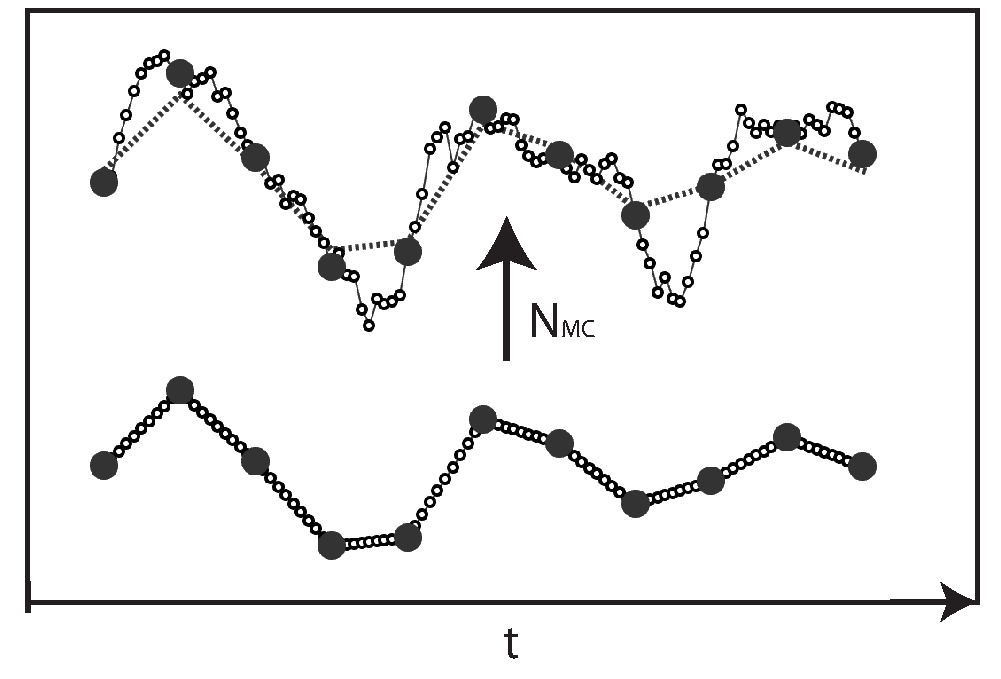
\includegraphics[width=0.7\textwidth]{FigPolymer2.pdf}
    \caption{Simulated polymer chain dynamics, with $n+1=11$ data points (large circles) and $j-1=9$ intermediate beads (small circles). For other parameters see Section~\ref{numerical_results}. Bottom: initial state, where intermediate beads are on a linear interpolation between data points. Top: polymer after $N_{MC}=1000$ iterations of the propagation algorithm (dotted line: initial configuration). Clearly the new configuration is mostly determined by the dynamics of the light-mass intermediate beads, while the heavy-mass data points move to a much lesser extent.}
    \label{fig:polymer}
\end{figure}

We have thus reduced the original Bayesian inference problem to simulating the dynamics of a linear polymer (cf. Fig.~(\ref{fig:polymer})). Each state of this fictitious molecule corresponds to a well-defined configuration in the original phase space, characterized by a set of system variables $\left\{q_i\right\}_{i=1,\dots,N}$ and a parameter vector $\bt$. It is now essential to note that potential (\ref{Vdisc}) contains terms of distinct scaling in the potentially large numbers $N$ and $n$, that refer to dynamics on distinct time-scales. In particular, for large $N$, $V(q,\bt)$ is dominated by its harmonic part, and to resolve its dynamics, brute force numerical integration of Hamilton's equations in step ($ii$) of the HMC algorithm would require a very small discretization time-step.

Whereas an interesting {\em approximative} approach would have been to employ a partial averaging of the fast Fourier modes \cite{doll_1985_fourier}, we will use an {\em exact multiple time scale integration} based on Trotter's formula \cite{tuckerman_1993}. For this, we introduce so-called {\it staging variables}, and diagonalize the harmonic part between the measurement points. To this end, we rewrite the discretized harmonic part of the action as
\begin{equation}
  \sum_{i=2}^{N}
  \frac{T}{2\Delta t}
  (q_i-q_{i-1})^2
  =
  \frac{T}{2}
  \sum_{s=1}^{n}\left\{
    \frac{(q_{(s-1)j+1} - q_{sj+1})^2}{j\Delta t}
    +
    \sum_{k=2}^j
    \frac{k}{(k-1)\Delta t}
    (q_{(s-1)j+k}-q^*_{(s-1)j+k})^2
  \right\}\,,
\end{equation}
with $  q^*_{(s-1)j+k}  =  ((k-1)q_{(s-1)j+k+1} + q_{(s-1)j+1} )/k$.
For the boundary beads, corresponding to the original measurement points, we apply the coordinate transformations
$  u_{sj+1} = q_{sj+1}$, $s=0,\dots,n$
and for the intermediate staging beads
$u_{sj+k} = q_{sj+k} - q^*_{sj+k}$, $s=0,\dots,n-1$, $k=2,\dots,j$.
Their inverse transformations are given by
\begin{align}
  q_{sj+1} &= u_{sj+1}\,,
  \\
  q_{sj+k} &= \sum_{l=k}^{j+1}\frac{k-1}{l-1}u_{sj+l}
  +\frac{j-k+1}{j}u_{sj+1}\,,
\end{align}
which can be captured by the recursive relation
\begin{equation}
  q_{sj+k} = u_{sj+k} + \frac{k-1}{k} q_{sj+k+1}+ \frac{1}{k}u_{sj+1} \,.
\end{equation}
We now split the Hamiltonian $\mathcal{H}_{\mbox{\tiny HMC}}$ into components according to their scaling behavior in $n$ and $N$, and write
\begin{equation}
  \mathcal{H}_{\mbox{\tiny HMC}}= \mathcal H_N+\mathcal H_n+\mathcal H_1\,,
\end{equation}
where
\begin{align}
  \mathcal H_N &=
  \frac{1}{2}
  \sum_{s=1}^{n}
  \sum_{k=2}^j
  \left\{
    \frac{\Delta t}{m'}p_{(s-1)j+k}^2
    +
    \frac{Tk}{\Delta t(k-1)}
    u_{(s-1)j+k}^2
  \right\}\,,\label{H_N}
  \\\label{H_n}
  \mathcal H_n &=
  \frac{1}{2}
  \sum_{s=1}^{n+1}
  \left\{
   \frac{\Delta t }{M}p_{(s-1)j+1}^2
    +
    \frac{(\ln(y_s/r_{(s-1)j+1}) - {\beta u_{(s-1)j+1}})^2}{\sigma^2}
   \right\}
   \\\nonumber
  &+
  \frac{T}{2j\Delta t}
  \sum_{s=1}^{n}
    (u_{(s-1)j+1} - u_{sj+1})^2
   \,,
  \\ \label{H_1}
  \mathcal H_1 &=
   \sum_{\alpha=1}^2\frac{\pi_\alpha^2}{2m_\alpha}
   +
  \frac{\Delta t}{T}
   \sum_{i=2}^{N}
   \left\{
    \frac{1}{2}
     \left(
        \rho_i-\frac{\beta}{\gamma}e^{-\beta q_i}
     \right)^2
    -
    \frac{\beta^2}{2\gamma}
    e^{-\beta q_i}
   -
    T q_i\dot\rho_i
   \right\}
  \\\nonumber
  &+
  \frac{1}{\gamma}
  e^{-\beta q_N}
  +
  q_N \rho_{N}
  -
  \frac{1}{\gamma}
  e^{-\beta q_1}
  -
  q_1 \rho_{2} \,.
\end{align}

Here, we have introduced two masses, $M$ and $m'$, for the boundary and staging beads, respectively.
For the staging beads, the harmonic part of Eq.~(\ref{H_N}) scales linearly with $N$. The terms of Eq.~(\ref{H_n}), including both the harmonic part for the boundary beads and the measurement term, scale linearly with $n$. Finally, Eq.~(\ref{H_1}) neither scales with $n$ nor $N$.
Thanks to the staging variables, $\mathcal H_N$ and $\mathcal H_n$ have become fully decoupled.
We use Trotter's formula \cite{tuckerman_1992} in order to design a reversible molecular dynamics integrator that takes the presence of the different time scales into account.
For an appropriate partition of the Hamiltonian, three distinct regimes can be distinguished:

 \begin{enumerate}
   \item[\it (i)]
  $\mathcal H_N \sim \mathcal H_n >> \mathcal H_1$,
  \item[\it (ii)]
  $\mathcal H_N >> \mathcal H_n \sim \mathcal H_1$,
  \item[\it (iii)]
  $\mathcal H_N >> \mathcal H_n >> \mathcal H_1$.
\end{enumerate}

In the following we restrict ourselves to regime $(ii)$, where the number of measurements $n$ is assumed to be not too large and/or the measurement error $\sigma$ to be not too small (the generalization of the method to the other regimes would, however, be straightforward). In this regime we may simply separate the harmonic part of the action for the staging beads from the rest and write
\begin{equation}
  \mathcal{H}_{\mbox{\tiny HMC}}=\mathcal H_N + \mathcal H'\,.
\end{equation}
For obtaining reversible integrators, we define the Liouville operators
$ iL_N=\{\cdot\,,\,\mathcal H_N\}$, $iL'=\{\cdot\,,\,\mathcal H'\}$,
where $\{\cdot\,,\,\cdot\}$ denote the Poisson brackets that apply to functions on the phase space.
Trotter's formula \cite{trotter_1959} allows us to write the Hamiltonian propagator as
\begin{equation}\label{propagator}
  e^{i(L_N+L')\tau}
  =
  (e^{iL_N(\Delta\tau/2)}e^{iL'\Delta\tau}e^{iL_N(\Delta\tau/2)})^P
  +
  \mathcal O(\tau^3/P^{2})\,,
\end{equation}
for $\tau =P\Delta \tau$.
Here, the outer propagator $\exp[iL_N(\Delta \tau/2)]$ reflects much faster dynamics than the inner one.
However, thanks to our re-parametrization, it describes the dynamics of uncoupled harmonic oscillators, which we can readily solve.
Masses and frequencies of the oscillators are derived from (\ref{H_N}) as
\begin{equation}
  m=m'/\Delta t\,,\quad
  \omega_k=\sqrt{\frac{Nk}{(k-1)m}}\,.
\end{equation}
The outer propagator becomes
\begin{align}
  u_{(s-1)j+k}(\Delta\tau/2)
  &=
  u_{(s-1)j+k}(0)\cos(\omega_k\Delta\tau/2)
  +
  \frac{p_{(s-1)j+k}(0)}{m\omega_k}\sin(\omega_k\Delta\tau/2)\,,
  \\
  p_{(s-1)j+k}(\Delta\tau/2)
  &=
  p_{(s-1)j+k}(0)\cos(\omega_k\Delta\tau/2)
  -
  m\omega_k u_{(s-1)j+k}(0) \sin(\omega_k\Delta\tau/2)\,,
\end{align}
for $s=1,\dots,n$ and $k=2,\dots,j$.
This elegant `analytical' solution is one main boosting part of our algorithm.
For the inner propagator, we employ the time-reversible and volume preserving velocity Verlet algorithm \cite{swope_1982_verlet}, which leads for the boundary beads to
\begin{align}
  u_{(s-1)j+1}(\Delta\tau)
  &= u_{(s-1)j+1}(0)
  +
  \frac{\Delta\tau}{M} p_{(s-1)j+1}(0)
  +
  \frac{\Delta \tau^2}{2M}
  F_{(s-1)j+1}[\vc u(0),{\pmb\theta}(0)]\,,\\
  p_{(s-1)j+1}(\Delta\tau)
  &= p_{(s-1)j+1}(0)
  +
  \frac{\Delta\tau}{2}
  (
  F_{(s-1)j+1}[\vc u(0),{\pmb\theta}(0)]
  +
  F_{(s-1)j+1}[\vc u(\Delta\tau),{\pmb\theta}(\Delta\tau)]
  )\,,
\end{align}
with $s=1,\dots,n+1$ and where $F_i[\vc u,{\pmb\theta}]$ denotes the partial derivative of $\mathcal H'[\vc u,{\pmb\theta}]$ w.r.t. $u_i$.
Analogous equations emerge for the model parameters $\bt$ and their momenta ${\pmb\pi}$, by exchanging $u_{…}$ by $\theta_{…}$ and $p_{…}$ by $\pi_{…}$, along with the corresponding masses, respectively.
For the staging beads
%, as yet another benefit of the approach,
only the momenta need to be updated (because the associated kinetic term is not part of $\mathcal H'$, but of $\mathcal H_N$).
Thus, with $s=1,\dots,n$ and $k=2,\dots,j$ as before,
\begin{align}
  p_{(s-1)j+k}(\Delta\tau)
  &=
  p_{(s-1)j+k}(0)
  +
  \frac{\Delta\tau}{2}
  (
  F_{(s-1)j+k}[\vc u(0),{\pmb\theta}(0)]
  +
  F_{(s-1)j+k}[\vc u(\Delta\tau),{\pmb\theta}(\Delta\tau)]
  )
  \,.
\end{align}

The propagators (28)-(32) are applied sequentially $P$ times to calculate the system evolution over time $\tau$. The proposed configuration, $(\vc u',\bt';\vc p',{\pmb\pi}')$ is accepted with Metropolis probability $  \min
  \left(
    1,
    e^{\mathcal{H}_{\mbox{\tiny HMC}}(\vc u,\bt;\vc p,{\pmb\pi}) - \mathcal{H}_{\mbox{\tiny HMC}}(\vc u',\bt';\vc p',{\pmb\pi}')}
  \right)$.
The next iteration then starts with sampling a new momentum vector $(\vc p,{\pmb\pi})$.

\section{Results}\label{numerical_results}

For our toy system, we have considered a simple sinusoidal input  $r(t) = \sin^2 \left( 0.01 t \right) + 0.1$. A system realization was first obtained from Eq.~(\ref{sde}) using $K_{\mbox{\small true}} = 50$ and $\gamma_{\mbox{\small true}}=0.2$.
Such system realization was then used to generate a synthetic time series of observed data according to Eq.~(\ref{data}). The error $\sigma$ was set to $0.1$. The input signal, the "true" system realization and the corresponding data time series are shown in Fig.~(\ref{fig:rain_data_S}).
%Since we are working with rescaled equations, all results are shown in arbitrary units of time.
\begin{figure}[htb!]
    \centering
    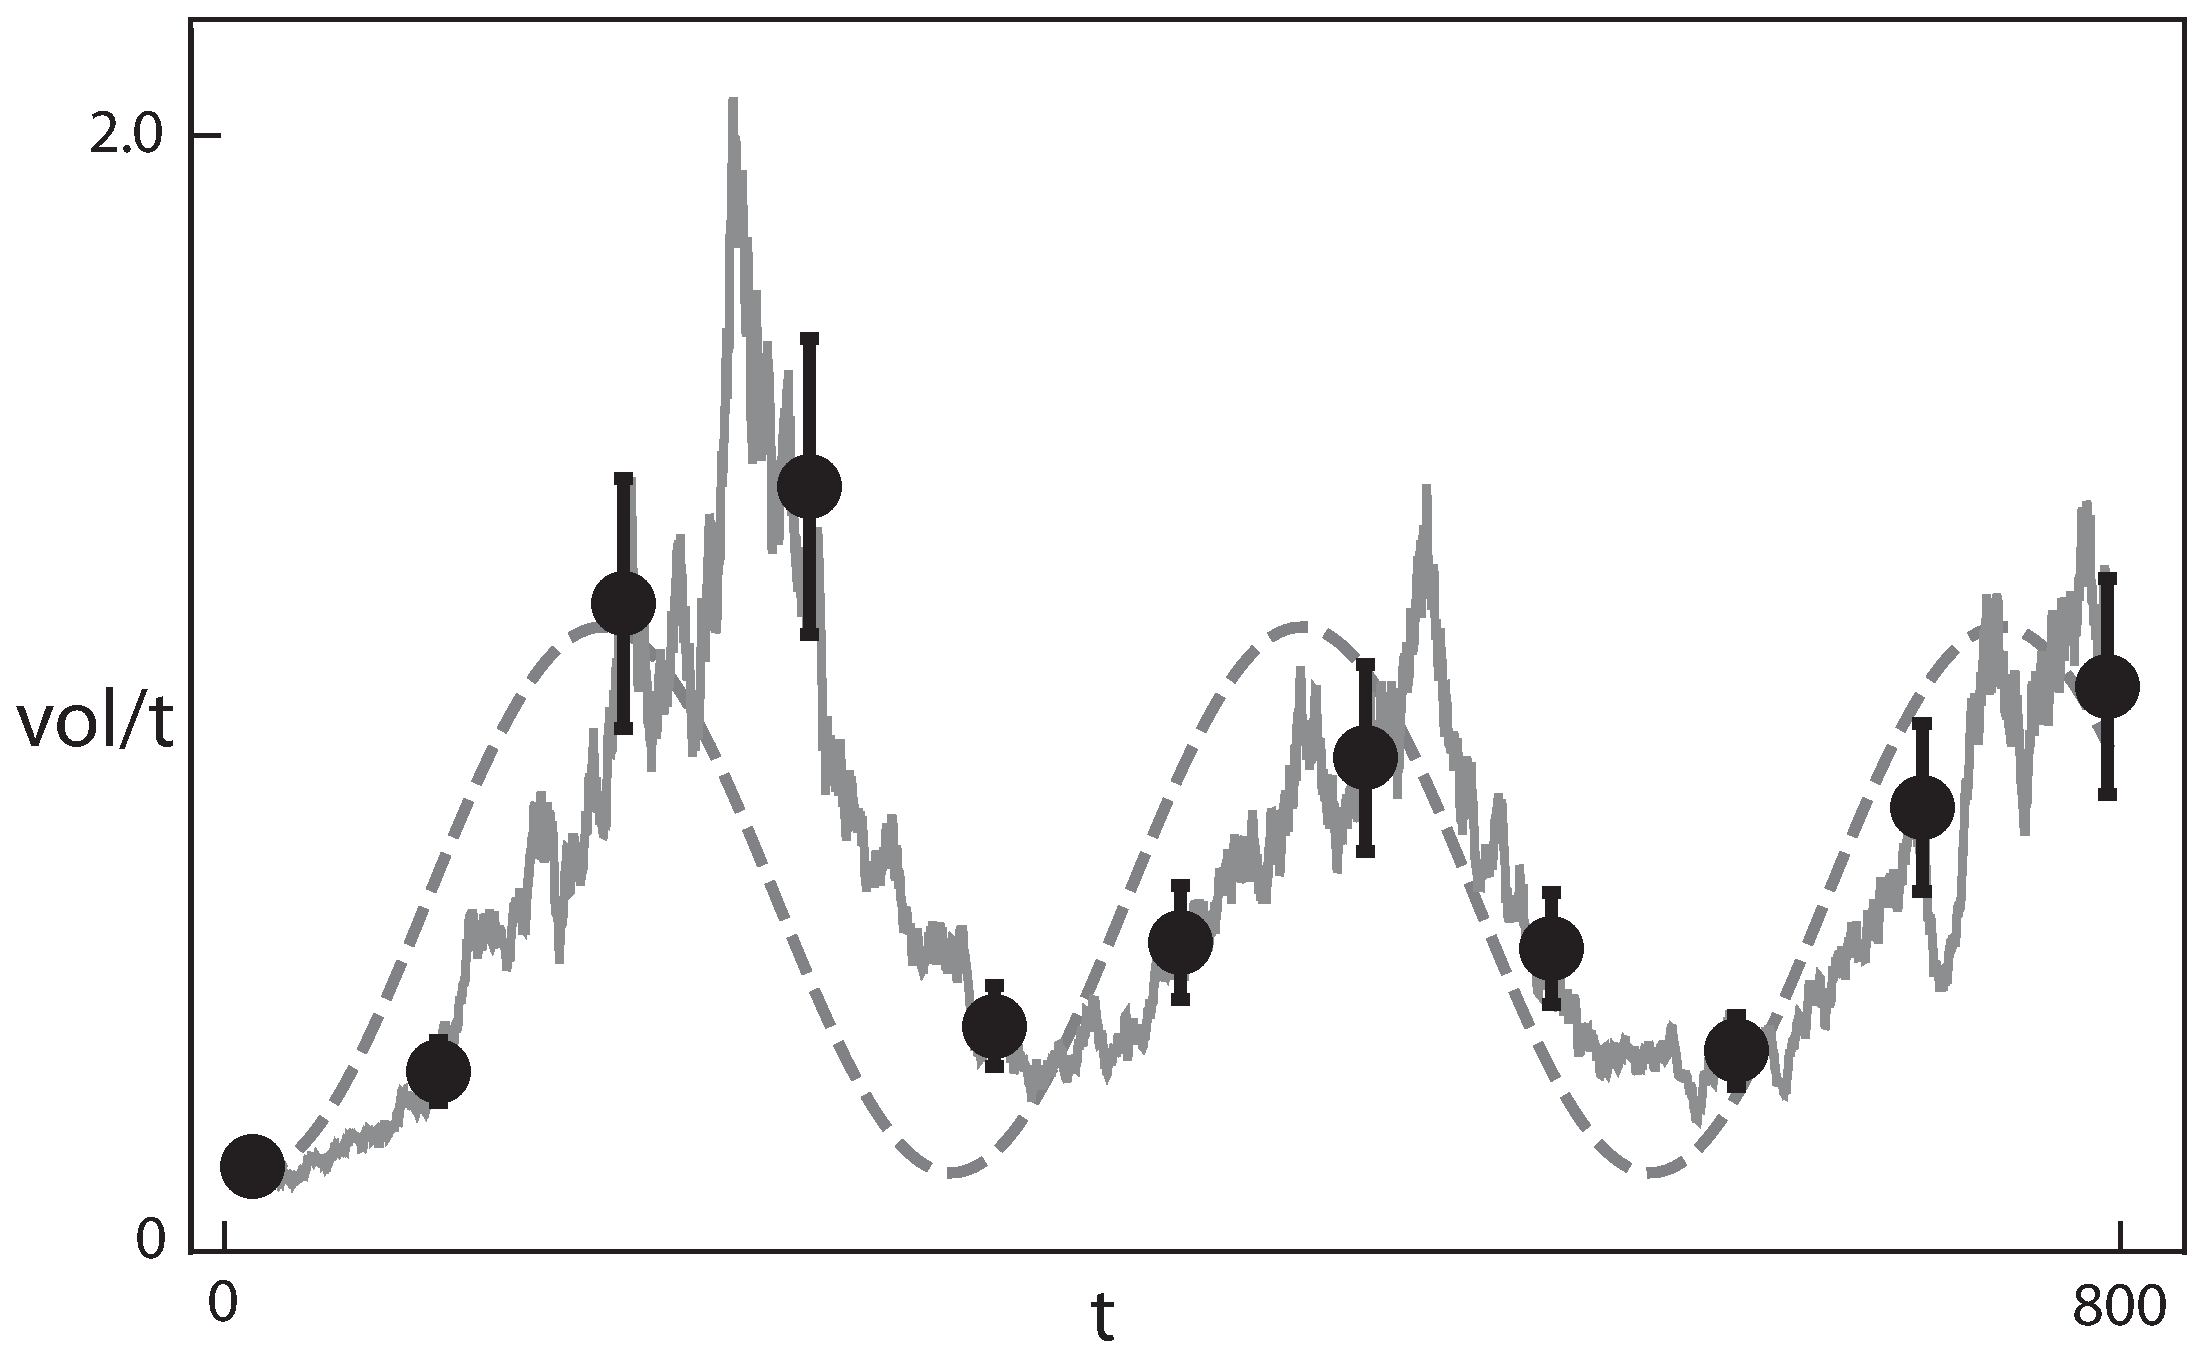
\includegraphics[width=0.7\textwidth]{Fig2.pdf}
    \caption{\label{fig:rain_data_S}
    System realization (solid line) with synthetic observations (filled circles, with error bars indicating the assumed measurement uncertainty).
    The system response closely follows the oscillations of the sinusoidal input (dashed) in a time-delayed manner.
    Parameters for this figure and all following figures: $K_{\mbox{\small true}} = 50$ and $\gamma_{\mbox{\small true}} = 0.2$.
%    Measured system realization (filled circles) and synthetic observed data (solid line and deviation bars attached to the circles evaluated across a longer time interval.). The system response closely follows time-delayed the oscillations of the sinusoidal input (dashed), with larger error bars where the prediction is less faithful. Parameters for this figure and all following figures: $K_{\mbox{\small true}} = 50$ and $\gamma_{\mbox{\small true}} = 0.2$.
}
\end{figure}
A complete run with 20000 iterations with $n=10$ and $j=30$ (i.e., $N = 301$ discretization points) required only about 40 seconds (for implementation details see the next section). A set of 200 simulated system realizations based on $j=30$ is shown in Fig.~(\ref{fig:spaghetti}), together with the generated synthetic data. In the simulation, the masses were set (in arbitrary units) to $M=720$ for the boundary beads, to $m=130$ for the staging beads, and to $m_\alpha=150$ for both the dimensionless parameters $\beta$ and $\gamma$. The different dynamics of the heavy boundary beads and the light staging beads can be appreciated in Fig.~(\ref{fig:spaghetti}).
%
\begin{figure}[htb!]
    \centering
    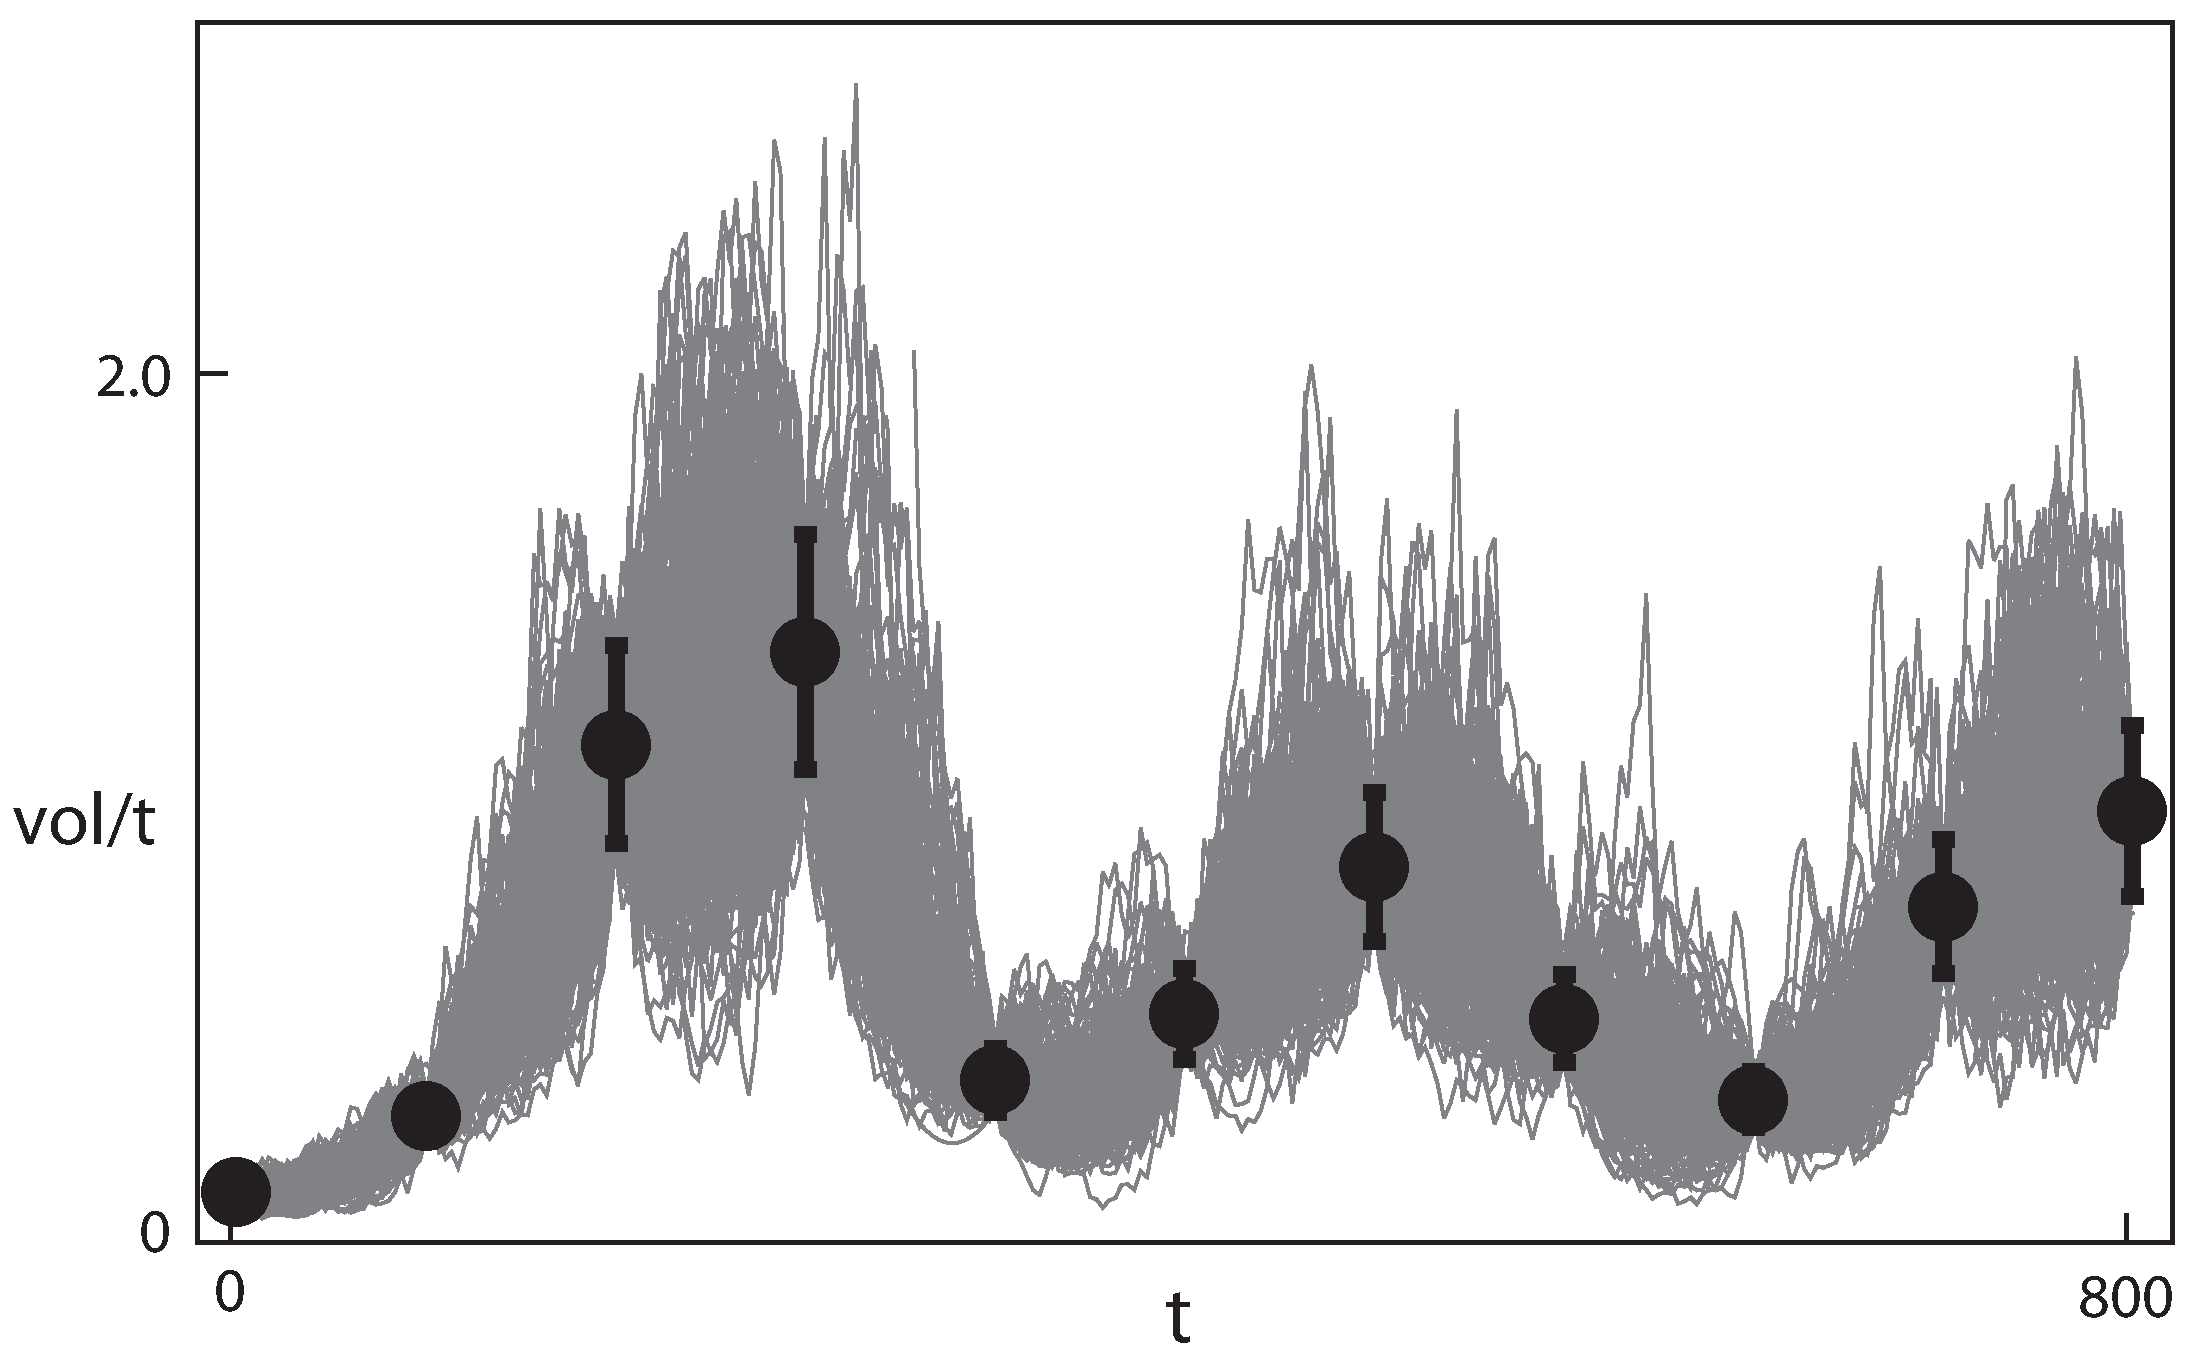
\includegraphics[width=0.7\textwidth]{Fig3.pdf}
    \caption{Simulated system realizations associated with synthetic data, based on $n+1 = 11$ measurement points, $j=30$ staging beads and  $N=301$ discretization points.
    %In the inset one may appreciate the different dynamics of heavy data points vs. the lighter staging beads.
}
    \label{fig:spaghetti}
\end{figure}
The Markov chains for parameters $K$ and $\gamma$, obtained after 50000 iterations of the HMC algorithm, are shown in Figs.~(\ref{fig:chainK}) and (\ref{fig:chainG}), respectively; they are fully compatible with the true, to be inferred, parameter values $K_{\mbox{\small true}}$ and $\gamma_{\mbox{\small true}}$.



\begin{figure}[htb!]
    \centering
    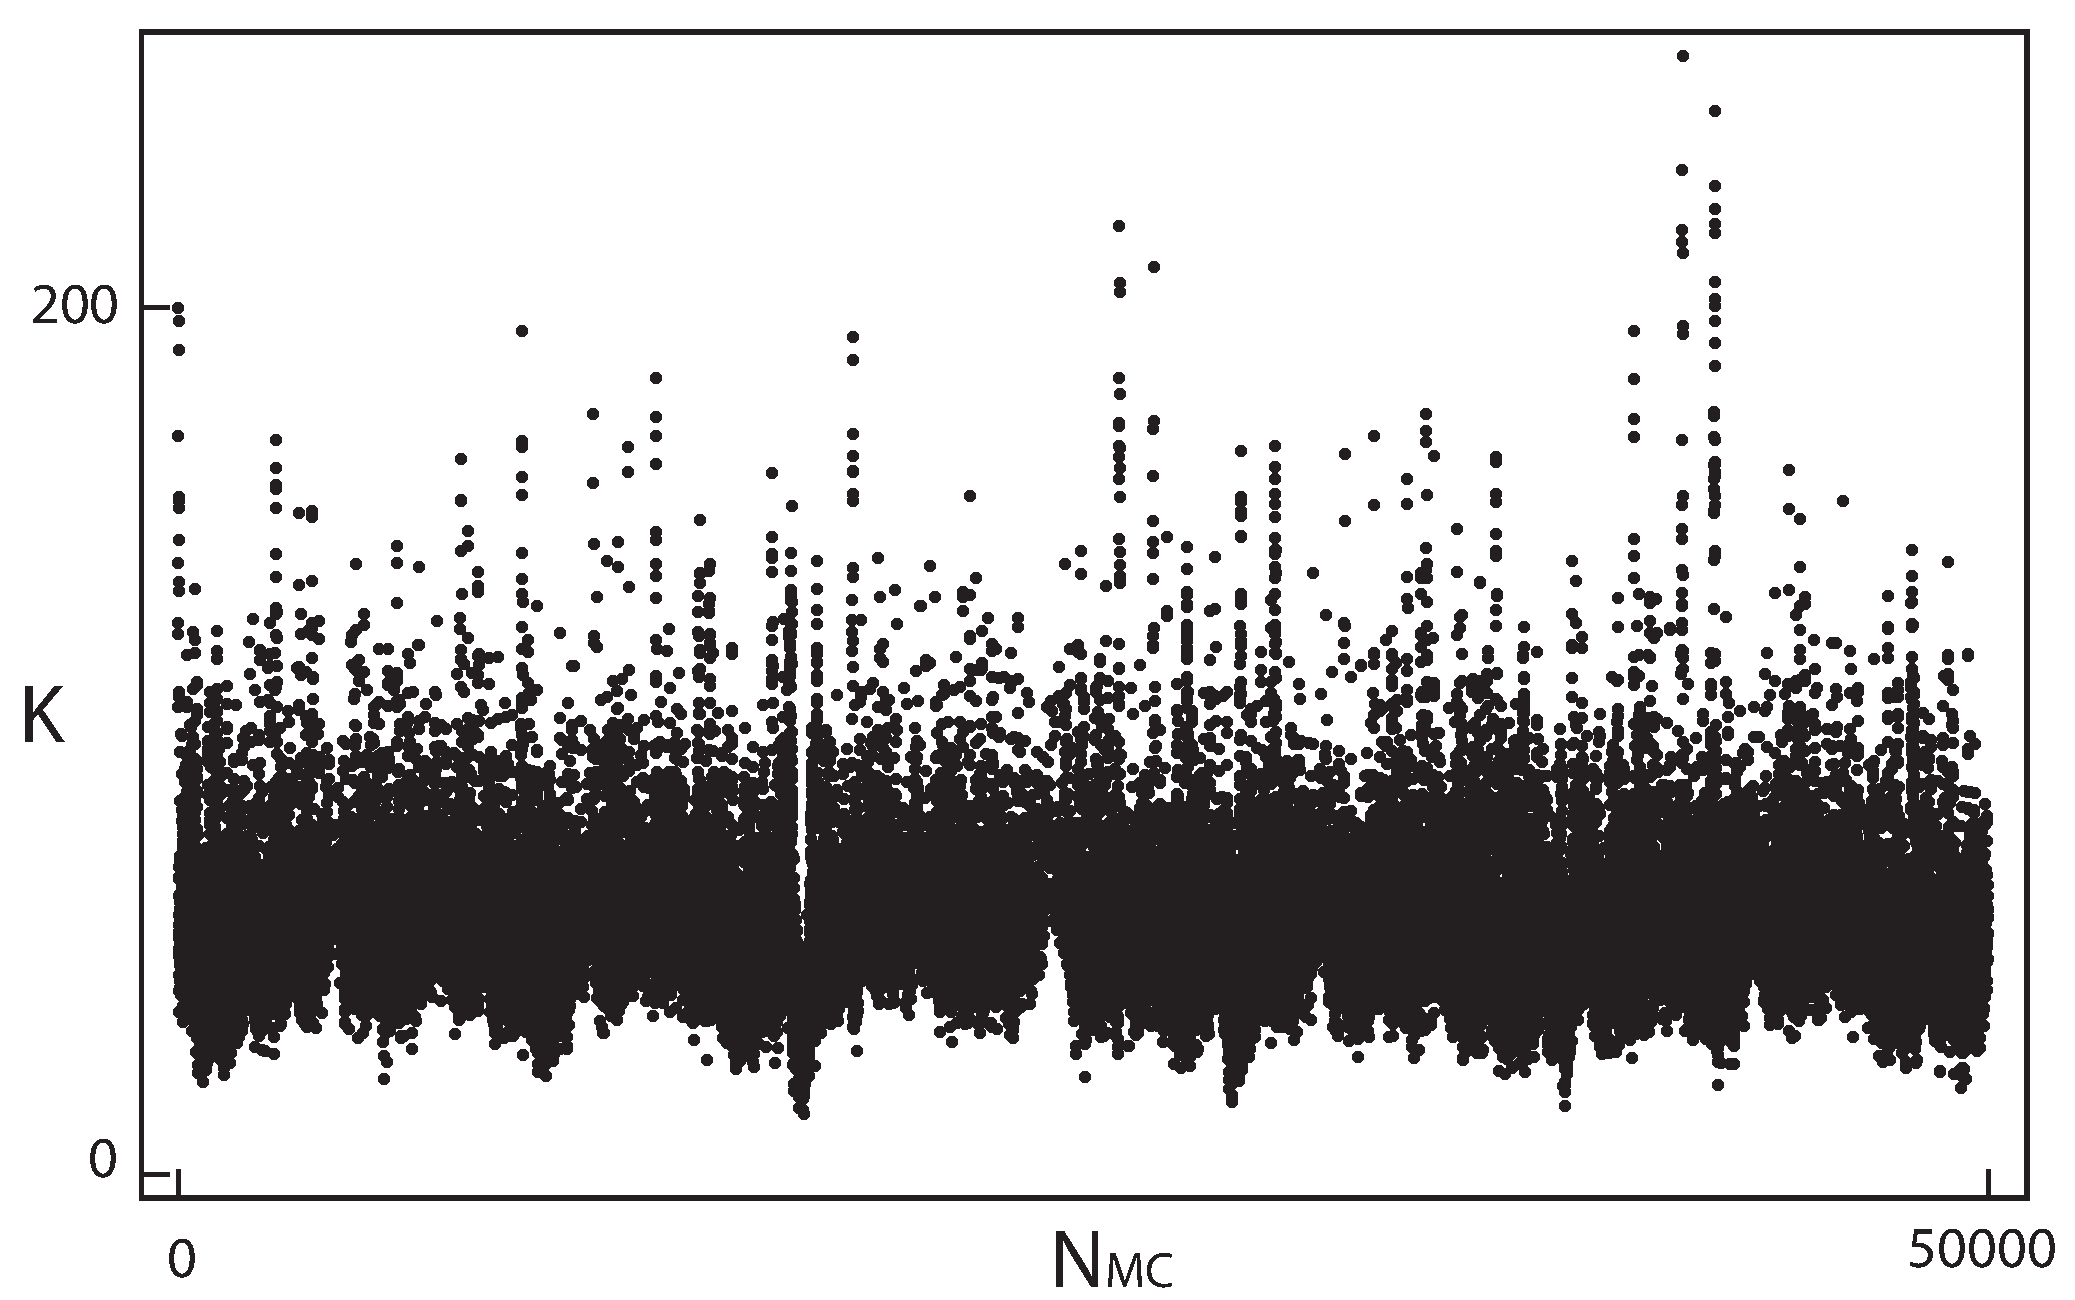
\includegraphics[width=0.7\textwidth]{Fig4.pdf}
    \caption{Markov chain evolution of the inferred parameter $K$.}
    \label{fig:chainK}
\end{figure}
%
\begin{figure}[htb!]
    \centering
    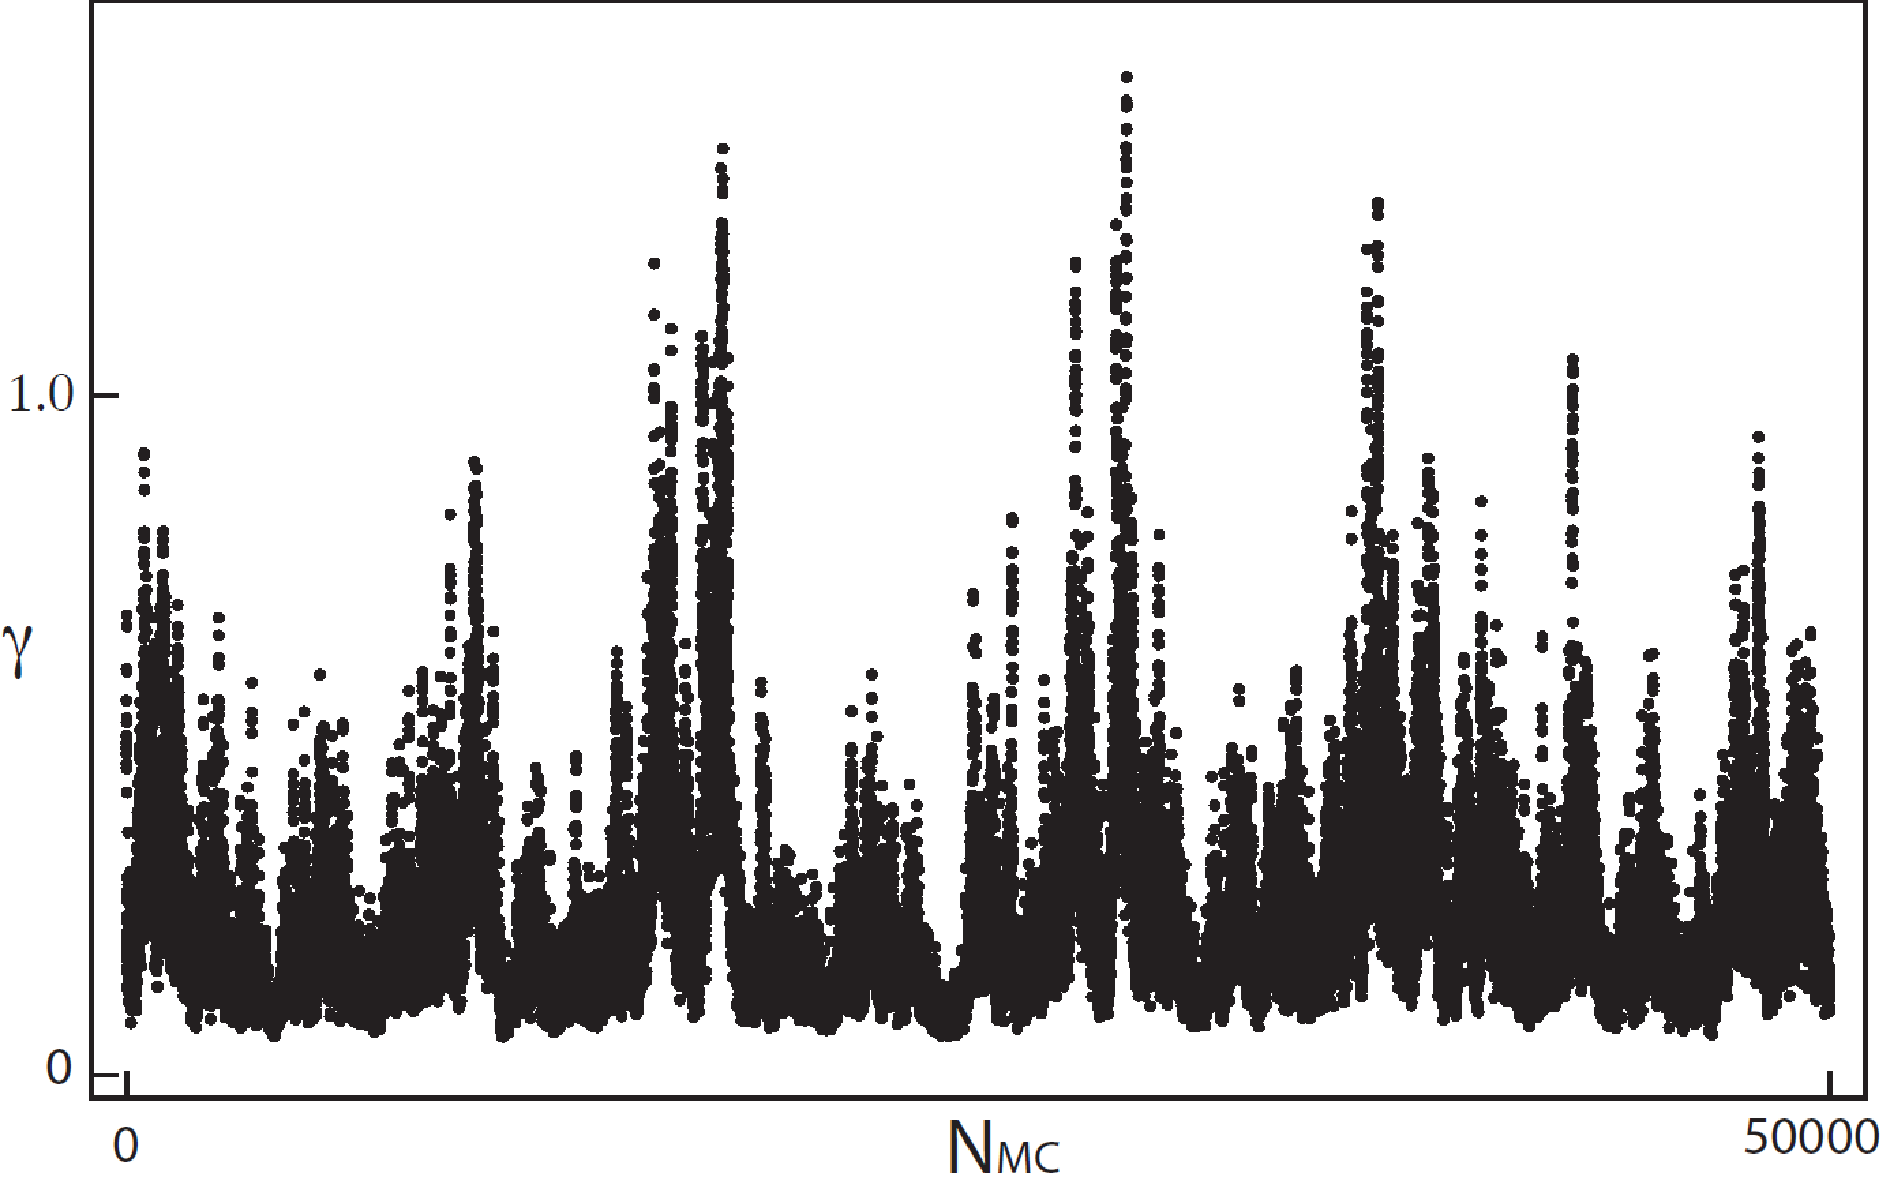
\includegraphics[width=0.7\textwidth]{Fig5.pdf}
    \caption{Markov chain evolution of the inferred parameter $\gamma$.}
    \label{fig:chainG}
\end{figure}

%\begin{figure}[htb!]
%    \centering
%    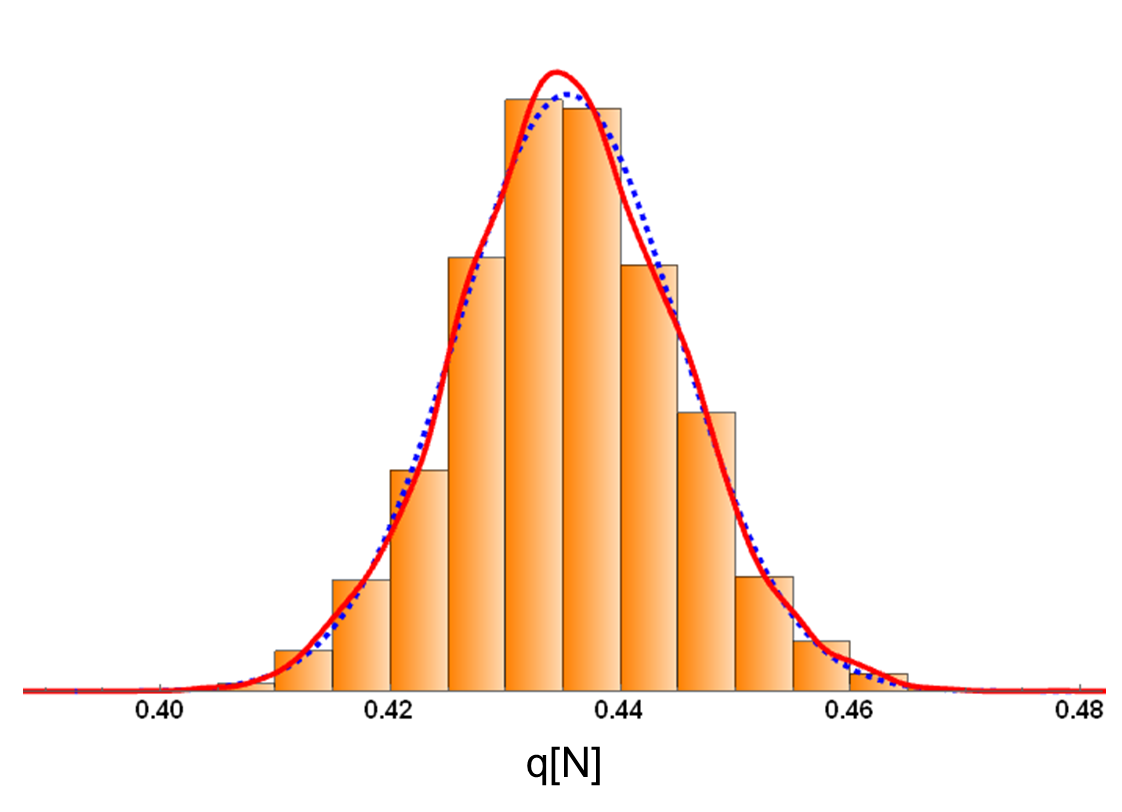
\includegraphics[width=0.3\textwidth]{FigFinalState.png}
%    \caption{PDF for the system final state expressed via the coordinate set $\left\{ q_N \right\}$. The dashed curve represents a normal distribution with the same mean and variance. The final state is basically normally distributed.}
%    \label{fig:final_state}
%\end{figure}
%
The efficiency of the algorithm can be appreciated best by inspecting the system evolution in the phase space $K-\gamma$ (Fig.~(\ref{fig:phase_space_evol})). The very first step of the algorithm already takes the system to the vicinity of the true parameter values, where most of its dynamics then occurs. Few excursions lead far away from the true parameter values. These explore the heavy tails of the posterior parameter distribution.
\begin{figure}[htb!]
    \centering
    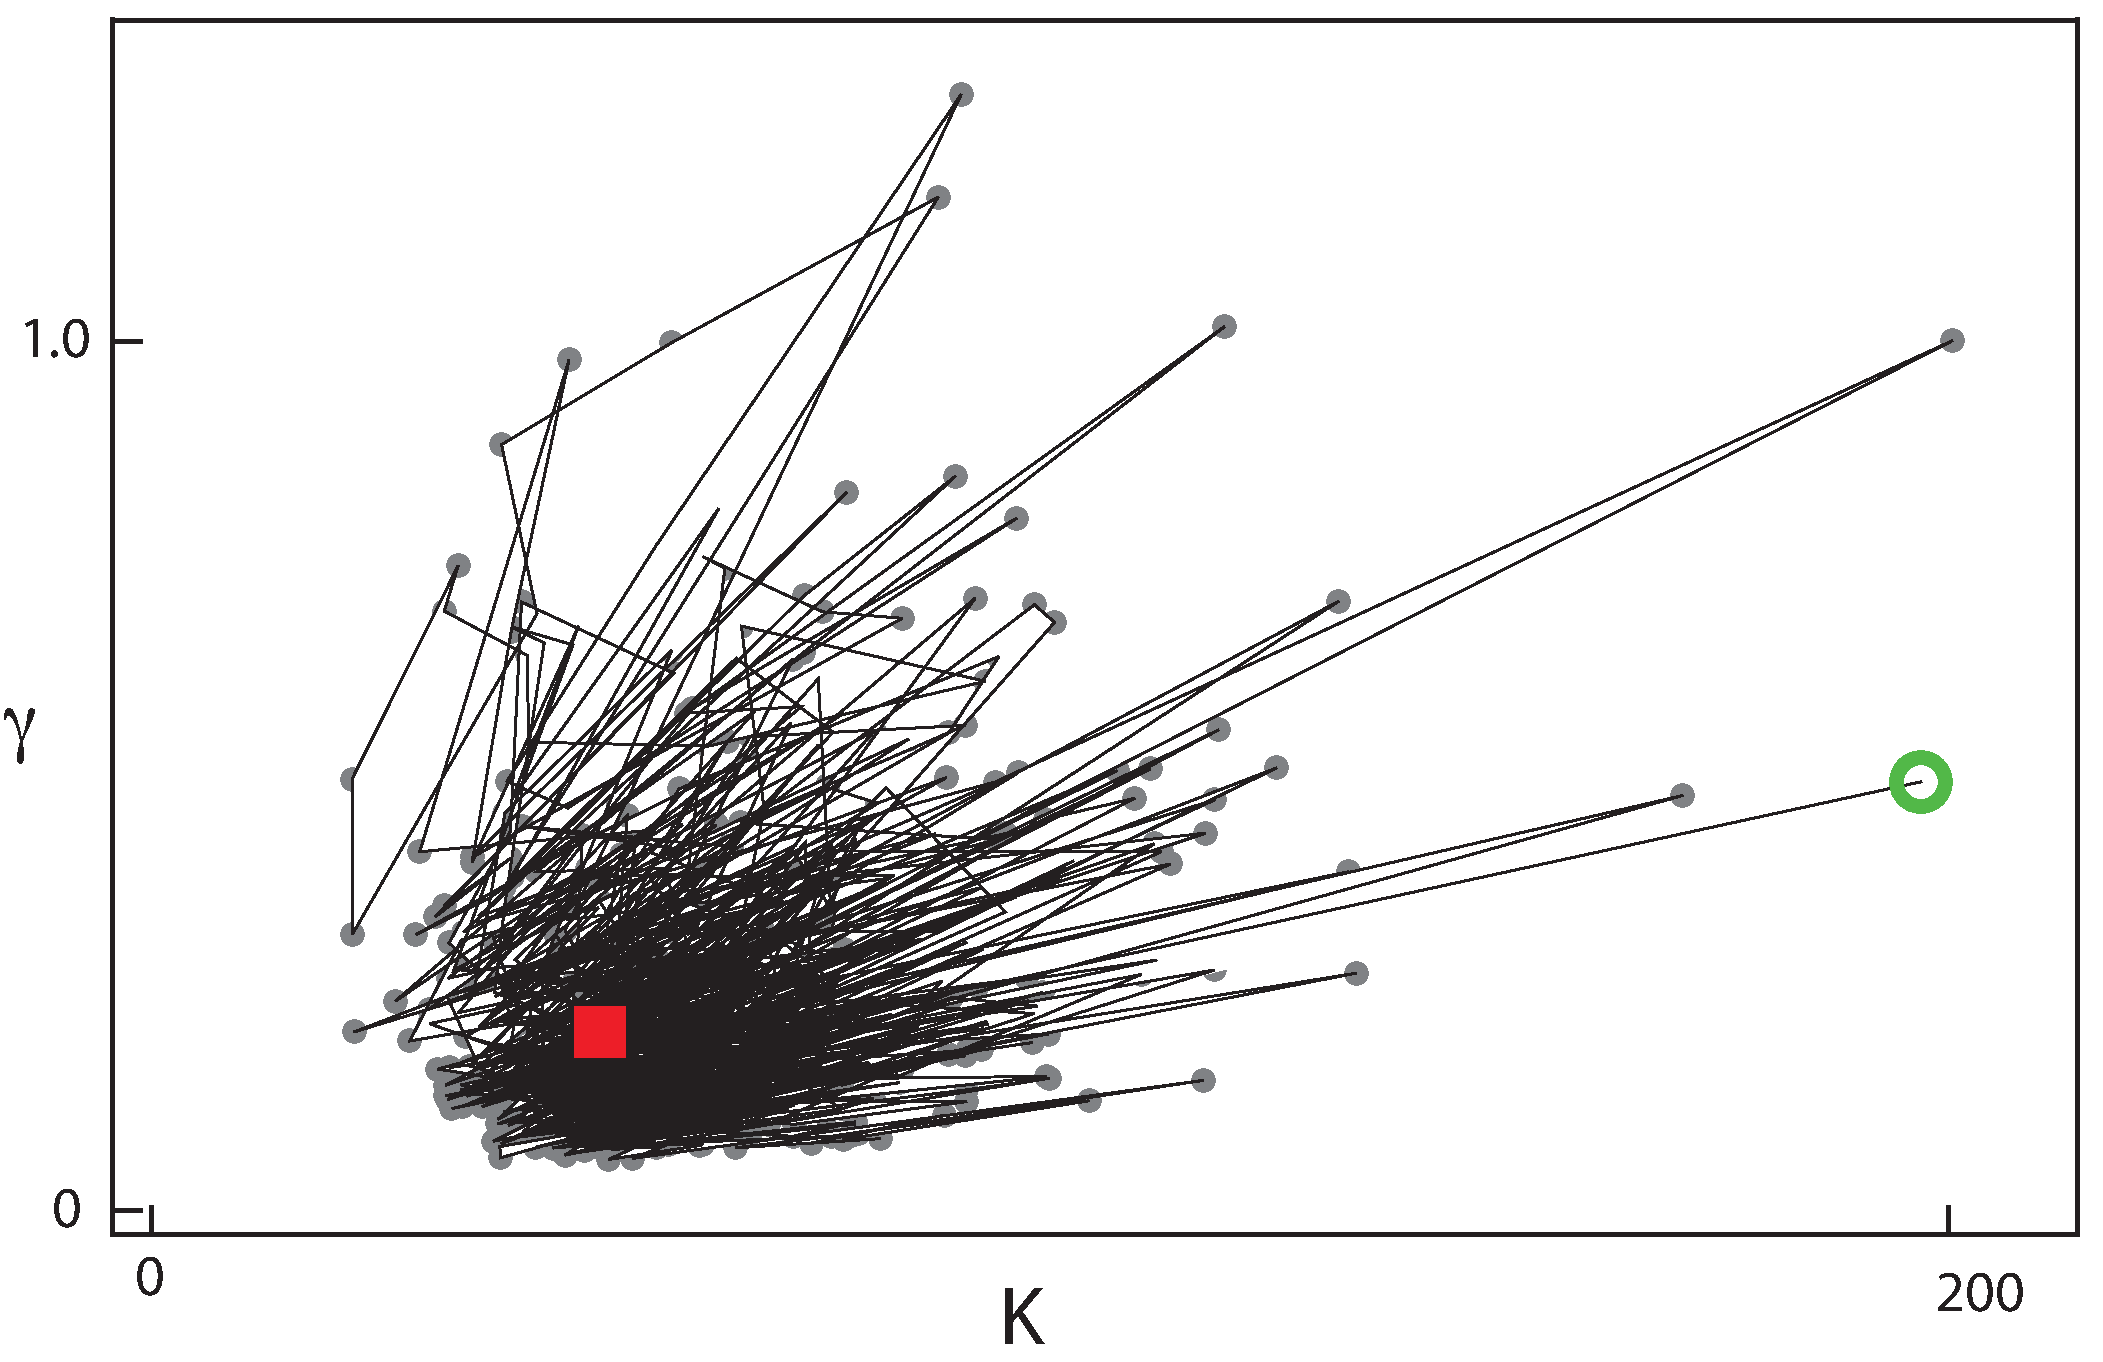
\includegraphics[width=0.7\textwidth]{Fig6.pdf}
    \caption{System dynamics in the phase space $K-\gamma$. The green circle represents the initial state, while the red square corresponds to the true parameter values used to generate the data.}
    \label{fig:phase_space_evol}
\end{figure}

The Markov chains (Figs.~(\ref{fig:chainK}) and (\ref{fig:chainG})) determine the probability density functions (PDF) for $K$ and $\gamma$, respectively. The result obtained by using the built-in kernel density estimator provided by Mathematica (version 10) is exhibited in  Fig.~(\ref{fig:KG_distr}).

\begin{figure}[htb!]
    \centering
    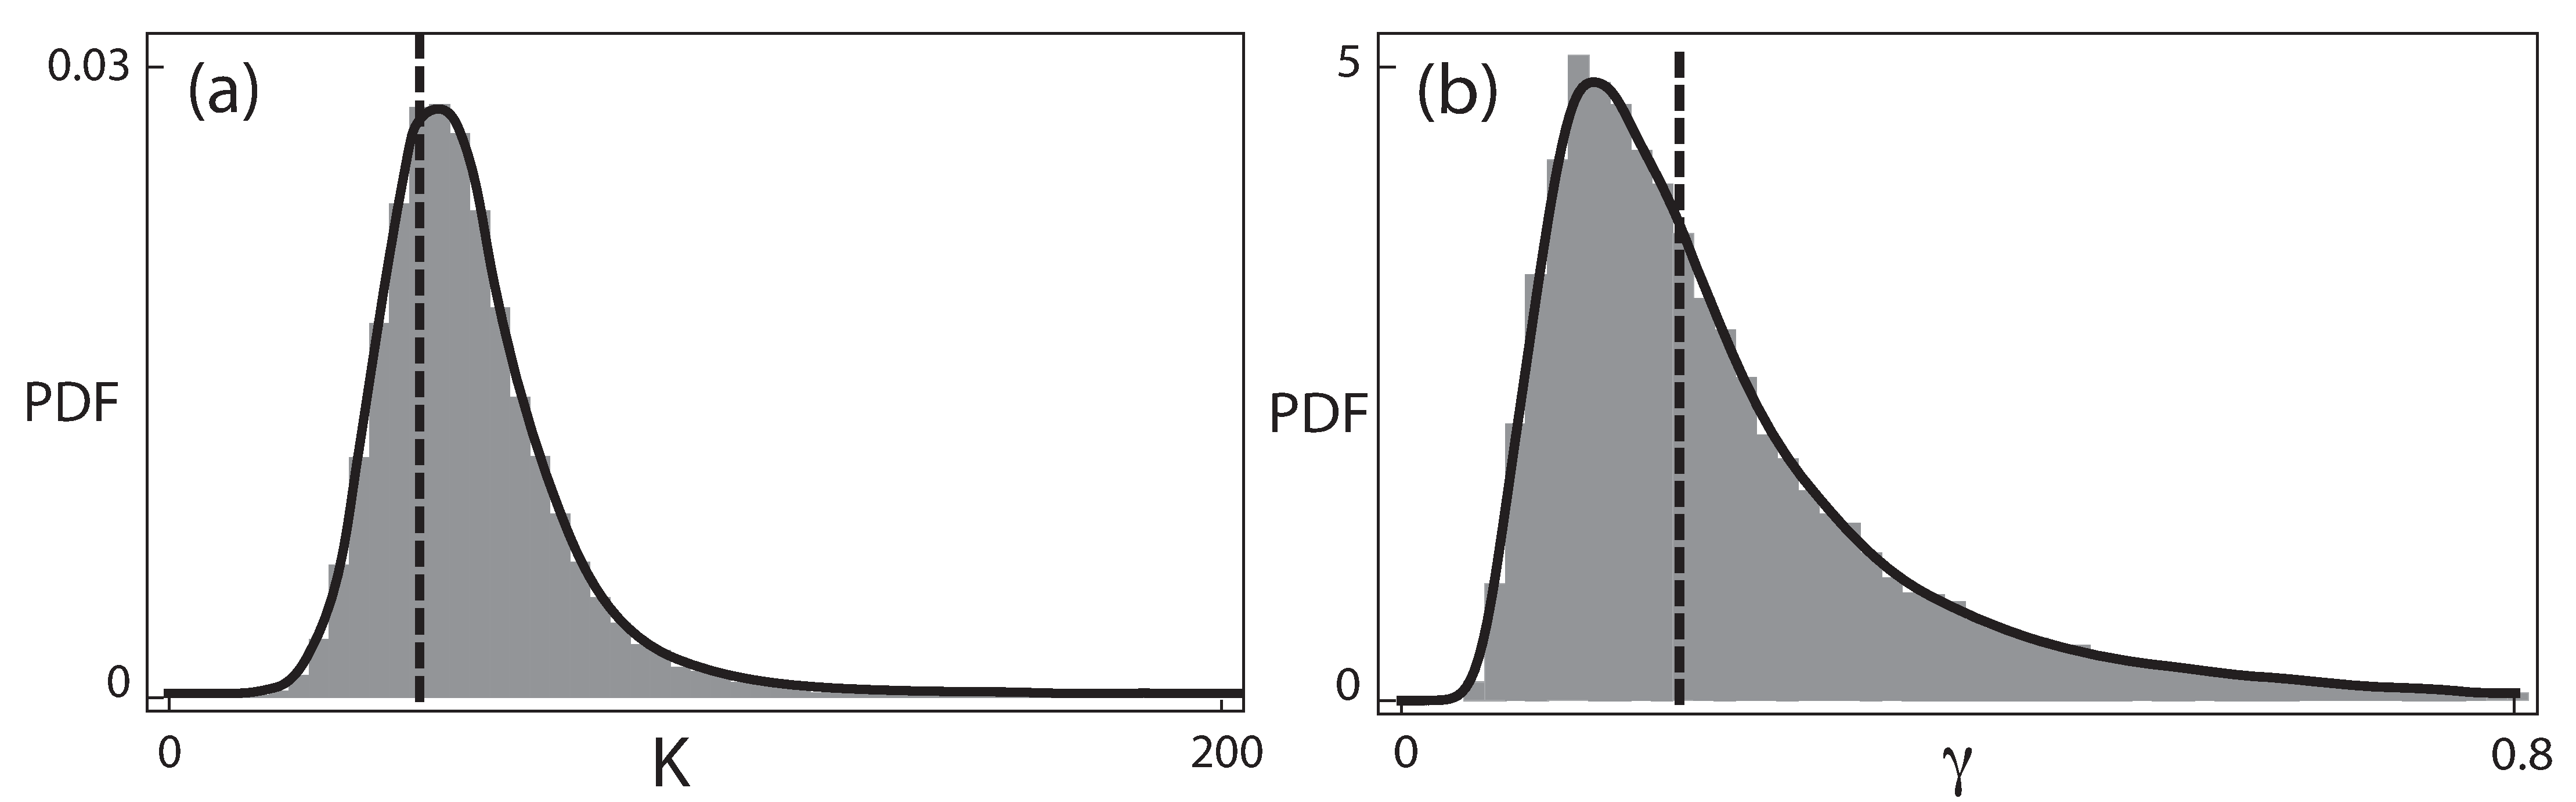
\includegraphics[width=1.0\textwidth]{Fig77.pdf}
    \caption{Probability density functions for the inferred parameters, (a) $K$ and  (b) $\gamma$. The true values used to generate the data are represented by the dashed vertical lines.}
    \label{fig:KG_distr}
\end{figure}


\section{Physical computational implementation}

The algorithm was implemented in C++ (version C++11) using the open source \emph{Adept} library (version 1.1)~\cite{Hogan_2014_adept}, which provides a powerful tool for fast reverse-mode automated differentiation (AD). Our algorithm benefits greatly from the use of AD. This gives us the possibility to modify Eq.~(\ref{sde}) and therefore the action~(\ref{action}), while leaving the implementation of the algorithm unaltered. This makes our program extremely flexible and suitable for a much broader range of applications than the simple exemplary SDE model described here.
%

The simulations were run on a serial implementation of the algorithm on a 64-bit laptop computer equipped with a Windows 7 operating system, a double-core 1.6~GHz CPU (Intel i5-4200U) and 8~GB of RAM. We used $n+1 = 11$ measurement points and $j = 10, 20,\dots, 50$ intermediate staging beads, with a total number of discretization points $N = 101, 201, \dots, 501$. In the Hamiltonian propagator~(\ref{propagator}), we set $\Delta\tau = 0.25$ and $P = 3$, with a constant total observation time $T = 833$ (arbitrary units of time).  Their initial values in the simulations were set to $K=200$ and $\gamma = 0.5$.
%



\section{Conclusions}

We presented a novel, extremely efficient and versatile approach for data-based SDE parameter estimation.
Our algorithm obtains its strength from translating the problem of generating posterior parameter samples into the problem of simulating the dynamics of a statistical mechanics system.
The main novelty in our algorithm is the exploitation of the fact that this dynamics generically happens on very different time scales.
Furthermore, at least for 1D systems, our approach also allows for an analytical, and therefore computationally efficient, integration of the fastest part of the dynamics.

Our algorithms works with a constant diagonal mass matrix, with reasonable choices of masses - heavier for the measurement beads, lighter for the discretization (staging) beads.
We expect this to work well in most application cases.
However, if the curvature of the potential varies strongly, it might be beneficial to adapt the mass matrix to the local curvature as suggested in Ref. \cite{girolami_2011_HMC}.
This, in turn, comes with some computational overhead, as second derivatives have to be calculated and implicit equations have to be solved.
Furthermore, we will no longer be able to solve part of the dynamics analytically.
Nonetheless, for certain applications, a combination of the scale separation method proposed in this paper with a local adaptation of the mass matrix from Ref. \cite{girolami_2011_HMC} might  be the most efficient approach.

%We presented a novel, extremely efficient and versatile approach for SDE parameter estimation, based on observed data. Compared to Ref. \cite{girolami_2011_HMC} that proposed an approach designed to remedy similar shortcomings of the traditional approaches, our approach is conceptually and implementation-wise much simpler and faster. Whereas for the former algorithm, locally the solution space metric needs to be evaluated, we only need to make reasonable choices of weights, heavier for the measurement beads, light for the staging beads. Although these choices are uncritical, they could be adapted to and optimized for the specific problem, if necessary. A particular advantage is that a large number of the updates can be done semi-analytically and do not involve the numerical calculation of derivatives. This saves a considerable computational effort.
%Our approach is much simpler to implement and to monitor, and should, according to the arguments provided, generally be faster.

The structure of our algorithm is well suited to parallelization, which is important in particular if we deal with a high number of measurements. The algorithm can easily be adapted to other inference problems, such as higher dimensional SDE, and SDE coupled to ODE. These adaptations and extensions will, however, be addressed in future works.



%\begin{figure}[htb!]
%    \centering
%    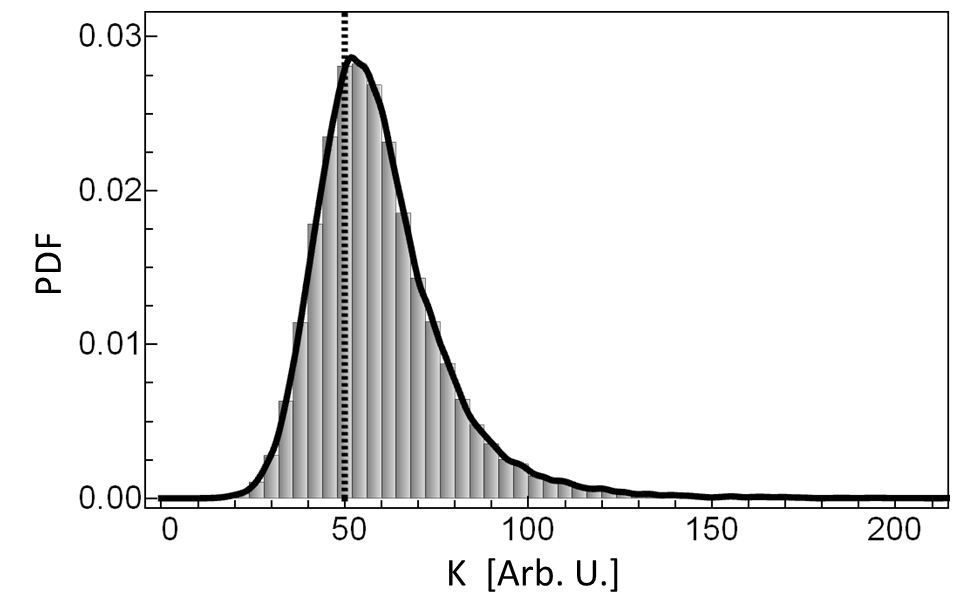
\includegraphics[width=0.7\textwidth]{FigK.png}
%    \caption{Probability density function for the inferred parameter $K$. The true value used to generate the data, $K_{\mbox{\small true}}=50$, is represented by the dotted vertical line.}
%    \label{fig:K_distr}
%\end{figure}
%
%\begin{figure}[htb!]
%    \centering
%    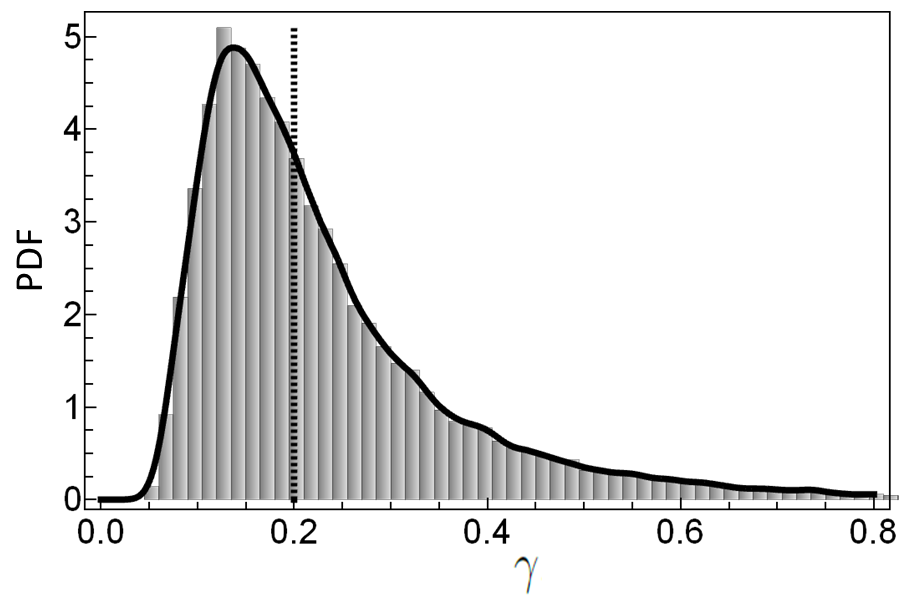
\includegraphics[width=0.65\textwidth]{FigG.png}
%    \caption{Probability density function for the inferred parameter $\gamma$. The true value used to generate the data, $K_{\mbox{\small true}}=50$, is represented by the dotted vertical line.}
%    \label{fig:G_distr}
%\end{figure}

%We tested the built-in Julia multiprocessing environment to run the program on two separate processes, but we observed a much slower performance compared to the serial implementation. This should not be surprising since with the small number of discretization points used so far, not more than a few hundreds, the overheads associated with the communication between the parallel processes significantly exceeded their advantages. Nevertheless, the method might be applied to systems requiring a much larger number of points. In hydrology, for instance, typical time series corresponding to hourly observations of precipitations and river discharges may contain several tens of thousands of measurements. In such cases a parallel version of the program would definitely improve the performance of the method. However, it is interesting to observe that Julia might not be the best option for parallelization. Indeed, the multiprocessing environment provided by Julia is strongly task oriented, while our problem is fundamentally data oriented. In view of a future parallelization of the HMC algorithm it is therefore advisable to investigate also alternative programming languages, such as C++. This issue will be discussed in a forthcoming publication.



\section*{Acknowledgement}
This work was partly financed by the Eawag Discretionary Fund.


\bibliographystyle{unsrt}
\bibliography{refs}


\end{document}

